\documentclass[journal]{IEEEtran}
% Shared look for the Rapport papers: packages and TikZ styles for the diagrams.
\usepackage[T1]{fontenc}
\usepackage{amsmath,amssymb}
\usepackage{graphicx}
\usepackage{booktabs}
\usepackage{tabularx}
\usepackage{array}
\usepackage{tikz}
\usetikzlibrary{arrows.meta,positioning,fit,backgrounds,calc,shapes.geometric,shapes.misc}
\usepackage{url}
\usepackage[hidelinks]{hyperref}
\graphicspath{{../figures/}}
\tikzset{
  >={Stealth[length=1.8mm]},
  box/.style={draw, rounded corners=2pt, align=center, font=\scriptsize, minimum height=7mm, inner sep=2pt, fill=#1},
  box/.default=cyan!8,
  code/.style={box=cyan!8},
  llm/.style={box=orange!12},
  io/.style={box=gray!10},
  unity/.style={box=green!10},
  bad/.style={box=red!8},
  good/.style={box=green!12},
  decision/.style={draw, diamond, aspect=2.2, align=center, font=\scriptsize, inner sep=1pt, fill=yellow!12},
  state/.style={draw, circle, align=center, font=\scriptsize, minimum size=12mm, fill=#1},
  state/.default=cyan!8,
  lab/.style={font=\tiny, align=center},
}
\newcolumntype{Y}{>{\raggedright\arraybackslash}X}


\begin{document}

\title{Rapport: A Code-Governed Digital Twin for an Embodied, On-Device Psychiatric Standardised Patient, with Paraphrase-Robust Memory and Three-Seed Held-Out Validation}

% Before submission: if paper 1 or 4 appears at a conference first, say so here and in the cover letter, and list what is new in this article.
\author{Faaz~Khan~Mohammad%
\thanks{F. K. Mohammad is with the Rapport project (e-mail: faazkhn1000@gmail.com).}}
\markboth{Preprint, November 2026}{Mohammad: Rapport, a Code-Governed Digital Twin for a Psychiatric Standardised Patient}

\maketitle

\begin{abstract}
Students learn psychiatric interviewing by practising with standardised patients, but trained actors are scarce and costly, and today's
language-model patients are mostly cloud text chats that invent symptoms and are unpredictable about suicidal thoughts. We present Rapport, a
spoken, embodied simulated psychiatric patient that runs entirely on one laptop, and its Digital Twin, a patient model in which ordinary code
makes every decision a clinician would want to check: what the doctor's sentence did, how trust and guardedness change, which memories are open,
and which behaviours are allowed. A single call to a local language model only puts that decision into words, and every sentence is checked
before it is spoken. Each patient is a data file, and the voice, face and body read the same decision. On 14 held-out conversations, each run
with three seeds and marked by a model from a different family, the Twin passed every safety gate: no jailbreaks, no portrayal failures, no
locked-memory leaks, and disclosure of suicidal thoughts whenever they were unlocked and asked about kindly. Its behaviour fitted the kind of
doctor more closely (top-two behaviour share 0.72 against 0.86) with unchanged accuracy (0.947 against 0.953). On a blind benchmark of 512 doctor
questions, hybrid keyword and sentence-embedding matching raised recall of reworded risk questions on the held-out half from 35.1\% to 72.7\%,
short of a 95\% target. The patient starts speaking a median 1.82\,s after the student stops, and examination requests were recognised in all 385
test sentences. Faculty ratings and a learner pilot are pending, and we report the shortfalls alongside the gains.
\end{abstract}

\begin{IEEEkeywords}
simulated patients, psychiatry education, standardised patients, large language models, patient modelling, embodied conversational agents,
semantic retrieval, safety, on-device AI, evaluation
\end{IEEEkeywords}

\section{Introduction}
\IEEEPARstart{T}{he} psychiatric interview is learned by doing. A trainee has to notice slow speech and a lowered gaze, ask open questions,
earn enough trust for a patient to admit that some nights they wish they would not wake up, and then assess risk properly, all inside a timed
examination station (an OSCE \cite{harden1975osce}). Actors trained as standardised patients make this practice possible, but they are costly,
not always available, and hard to keep consistent from one student to the next \cite{piot2021simulation}.

Large language models (LLMs) can play a patient, and many research systems now do
\cite{chen2023llmempowered,wang2024patient,lee2025psyche,sabour2026patientact,sabour2026patienthub,louie2024roleplaydoh}. A 2026
meta-analysis found that AI virtual patients help psychiatric interview training \cite{kilincel2026meta}. Five problems still stand between
these systems and an OSCE station:
\begin{itemize}
\item \textbf{The model makes things up.} Models invent symptoms or history to please the interviewer, more so under strong style cues
\cite{chen2023llmempowered}, and simulated patients agree too easily unless resistance is designed in \cite{steenstra2025scaffolding,lee2025psyche}.
\item \textbf{It is unpredictable where it matters most}, such as whether a patient admits suicidal thoughts, and nobody can see why it shared
or held something back.
\item \textbf{It misses questions asked in new words.} Students ask the same thing in many ways. A patient that fails to recognise a reworded
question about suicide may wrongly deny something it should share.
\item \textbf{It has no body and is too slow to talk to.} Psychiatric assessment depends on speech rate, pauses, face and posture, yet most
simulators are text chats \cite{wang2024patient,lee2025psyche,sabour2026patientact}, and rich patient agents use several model calls per turn.
\item \textbf{It runs in the cloud}, so a student's voice leaves the premises.
\end{itemize}

We take one route through all five: \emph{decide in code, voice with the model}. One model call per turn writes the words; everything a
clinician would audit is decided by code that we can read, test and change, and the body shows the same decision as the voice. This article
describes the whole system and its evaluation in one place.

\textbf{Contributions.}
\begin{enumerate}
\item \textbf{Rapport}, an on-device, spoken 3D standardised patient for psychiatry and addiction OSCEs, with four draft stations, four patient
bodies, seeded patients and six conversation styles, a live examiner view, physical examination on request, and a debrief grounded in the
assessment literature (Sections~\ref{sec:evidence}, \ref{sec:student} and \ref{sec:debrief}--\ref{sec:authoring}).
\item \textbf{An architecture} in which the patient is data, code decides, a local model speaks and the body reads the same decision, with
measured speed and the failures found on the way (Sections~\ref{sec:arch}--\ref{sec:data} and \ref{sec:results}).
\item \textbf{The Digital Twin}, a patient model whose state, memory locks, guardedness, allowed behaviours and consistency checks are explicit
code (Section~\ref{sec:model}).
\item \textbf{Paraphrase-robust recall}: a blind benchmark of 512 doctor questions with a strict tuning/test split, a hybrid matching method with
trust locks applied after matching, and training-free hand-set weights (Section~\ref{sec:recall}).
\item \textbf{A validation method and its results}: scripted held-out conversations on three seeds, a judge from another model family, a hand
check of every flag, an independent safety review, and feature ablations, reported with the targets the design missed
(Sections~\ref{sec:eval} and \ref{sec:results}).
\end{enumerate}

\section{Related Work}
\subsection{Psychiatric AI patients, and whether they help}


\textbf{Psychiatric AI patients.} Chen et al.\ built chatbots validated by clinicians for depression interviews \cite{chen2023llmempowered};
PATIENT-$\Psi$ bases patients on expert cognitive models with six conversation styles \cite{wang2024patient}; PSYCHE builds a Mental Status Exam
framework to evaluate assessment agents \cite{lee2025psyche}; PatientAct adds trust-gated memory, reactions and resistance \cite{sabour2026patientact};
PatientHub collects many simulators \cite{sabour2026patienthub}; Roleplay-doh lets experts steer a patient with written principles
\cite{louie2024roleplaydoh}. \textbf{Patients that learn.} EvoPatient improves patients through simulated doctor--patient practice and a checked
library of past replies \cite{du2024llms}; MedAgentSim and Agent Hospital evolve agents in simulated clinics \cite{almansoori2025selfevolving,li2024agent}.
\textbf{Patients with bodies and voices.} Design guidelines for psychiatric virtual patients predate language models \cite{dupuy2020guidelines};
recent language-model patients that act beyond text or appear as a lifelike avatar include Voigt et al.\ \cite{voigt2025llmpowered} and
SOPHIE \cite{haut2025ai}; SimPatient and MedSimAI add feedback
on the student's performance \cite{steenstra2025scaffolding,hicke2025medsimai}. \textbf{Does it help?} A randomised trial found that patient simulation
with structured feedback improved students' clinical decisions \cite{brugge2024llm}; AI scoring of OSCE interview transcripts agrees with experts
within one point 67--87\% of the time \cite{geathers2025benchmarking}; a 2026 meta-analysis supports AI virtual patients for psychiatric interview training
\cite{kilincel2026meta}. AI judges are cheap but biased \cite{zheng2023judging}. \textbf{Digital brains.} The Brain/MINDS Digital Brain programme
builds mathematical models of the brain from anatomical and physiological data \cite{brainminds}; the Twin is not a brain model, and borrows
only the general idea that responses change when expectations are not met.


\subsection{How well a language model holds a persona}

Studies of persona prompting point the same way. Prompted Big Five personalities show up in large models \cite{jiang2024personallm,serapio2023personality}. But self-report tests of a model's personality are unreliable. Three equivalent prompts give significantly different scores \cite{gupta2023selfassessment}. Re-ordering the questions alone moves scores by about a fifth of the scale, and a long conversation history makes small models \emph{less} stable \cite{tosato2025persist}. Instructions drift within about eight rounds of dialogue \cite{li2024instruction}. Persona variables explain under 10\% of the variance in human annotations, which limits how far a persona prompt can steer a simulation \cite{hu2024persona}. Model size does not predict how well a model keeps a persona \cite{samuel2025personagym}. And some traits, such as high psychopathy or low conscientiousness, are hard to produce by prompting at all \cite{lee2025trait}. Multi-turn reinforcement learning improves consistency
\cite{abdulhai2025consistent}, and interviews, not questionnaires, are the better way to test a role-playing agent \cite{wang2023incharacter}. For a 4-billion-parameter patient model, we drew one lesson. Personality and resistance must be held in code. The model should get one style label and a few example lines, not a list of trait scores.


\subsection{Matching questions to memories}


\textbf{Sentence embeddings.} Sentence-BERT made it practical to compare sentences by meaning, with one vector each \cite{reimers2019sentencebert}. MiniLM showed that small, distilled models keep most of the quality \cite{wang2020minilm}. Contrastive training (SimCSE, E5, the BGE family) is now the standard recipe for small general-purpose encoders \cite{gao2021simcse,wang2022e5,xiao2023cpack}. Dense retrieval matches questions to
passages the same way \cite{karpukhin2020dpr}, and benchmarks such as BEIR and MTEB showed that retrieval quality varies a lot from one domain to
another and must be measured in the target domain \cite{thakur2021beir,muennighoff2022mteb}. PAWS showed that models trained on easy paraphrase
pairs fail on pairs that share words but differ in meaning \cite{zhang2019paws}; our problem is the reverse, questions that share no words but
mean the same.

\textbf{Memory in simulated patients.} PatientAct gives each memory a trust level and activation cues \cite{sabour2026patientact}. AIPatient retrieves from a knowledge graph built from health records, with several agents per turn \cite{yu2024simulated}. Patient-Zero checks replies against single facts \cite{lai2025patientzero}. Generative agents retrieve memories by recency, importance and relevance \cite{park2023generative}.
These systems report end-to-end conversation quality, but none that we found reports how well the matching step itself survives rewording, or what
it costs when matching goes wrong on a risk topic. That is the gap this article addresses.


\section{How the Design Was Grounded in Evidence}\label{sec:evidence}
\textbf{Review method.} Before and during building, we reviewed 83 papers. They cover simulated patients, patient agents, learning simulators, how well models hold a persona, and how clinical interviews are assessed. 37 were read in full, 35 as abstracts, and 11 could not be reached (publisher paywall or not
found); none of the unreachable ones shaped a decision. For each paper we recorded what it could change in Rapport and gave a verdict: adopt
(1), adapt the idea (21), idea only (38) or skip (23). Code was reused only under permissive licences (MIT, Apache, BSD); papers whose code is
AGPL, non-commercial or unlicensed contributed ideas only. A second review covered personality, randomised patients and ward scenarios, and a
third covered how to assess the learner.

\textbf{What we took, and what we rejected.} Table~\ref{p4:tab:built} lists the main design choices with the evidence behind each. We deliberately rejected three ideas. Pipelines with several model calls per turn are too slow for spoken conversation. Fine-tuning on real or expert dialogues was out of scope, and no consented real data exists. Code under restrictive licences was not reused.

\begin{table}[t]
\caption{Design choices and the evidence behind them}
\label{p4:tab:built}
\centering
\scriptsize
\begin{tabularx}{\columnwidth}{@{}YY@{}}
\toprule
Evidence & What Rapport does\\
\midrule
Memories with trust levels, reactions and resistance labels \cite{sabour2026patientact} & Trust-locked memories; a locked memory gives
only a discomfort signal\\
``Feel first, speak second'' \cite{sabour2026patientact} & Behaviour and emotion are chosen before the words\\
Patients too agreeable unless resistance is designed \cite{steenstra2025scaffolding,lee2025psyche}; too rigid is unreal
\cite{bodonhelyi2025modeling} & Resistance 0--3 in code with softening rules\\
Mental Status Exam constructs and failure modes \cite{lee2025psyche} & A mental-status profile per case, enforced by code\\
Six conversation styles \cite{wang2024patient} & Seeded patients with one style per session\\
Check replies against single facts \cite{lai2025patientzero} & Every sentence checked against the case before it is spoken\\
Readable, slightly exaggerated cues from a fixed map; free-written cues get repetitive \cite{haut2025ai,bodonhelyi2025modeling} & A fixed
emotion-to-body map\\
Learn offline, keep a change only if a replay shows it helps \cite{du2024llms,li2024agent,agrawal2025gepa} & Versioned learning loop with gates
and rollback\\
Expert-written principles reduce awkward replies \cite{louie2024roleplaydoh} & Case-level principles in the prompt\\
Quote-based rubric feedback \cite{hicke2025medsimai} & Debrief comments quote the student's own lines\\
\bottomrule
\end{tabularx}
\end{table}

\textbf{Personality: vary the person, not the answer.} Persona prompting is fragile in small models: self-report personality scores shift with
question order and conversation history \cite{tosato2025persist}, and instructions drift within about eight rounds \cite{li2024instruction}.
So Rapport gives the model one conversation style with a few example lines, and holds the rest (trust steps, disclosure levels, length bands)
in code. Synthetic-patient generators such as Synthea build the full history first and render it afterwards \cite{walonoski2018synthea}; human
standardised-patient programmes likewise let several actors play one case while the case stays fixed. Rapport follows the same rule: a seed
changes the everyday details and the style, never the answer key.

\section{What a Student Experiences}\label{sec:student}

\begin{figure}[t]
\centering
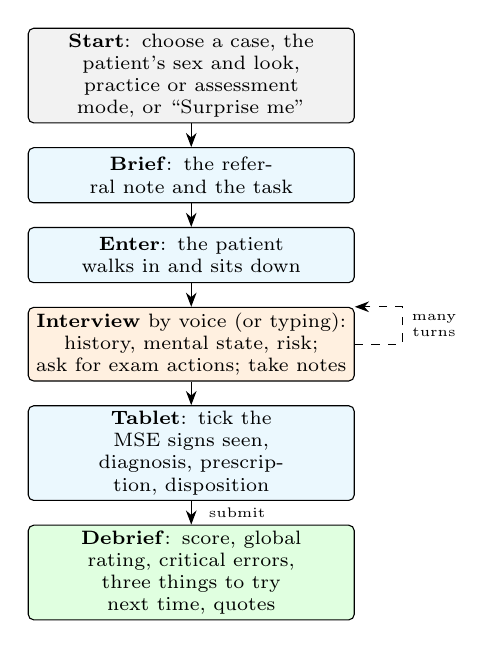
\begin{tikzpicture}[node distance=3mm]
\tikzset{b/.style={box=#1, text width=40mm}}
\node[b=gray!10] (s) {\textbf{Start}: choose a case, the patient's sex and look,\\practice or assessment mode, or ``Surprise me''};
\node[b=cyan!8, below=of s] (b) {\textbf{Brief}: the referral note and the task};
\node[b=cyan!8, below=of b] (e) {\textbf{Enter}: the patient walks in and sits down};
\node[b=orange!12, below=of e] (a) {\textbf{Interview} by voice (or typing):\\history, mental state, risk;\\ask for exam actions; take notes};
\node[b=cyan!8, below=of a] (t) {\textbf{Tablet}: tick the MSE signs seen,\\diagnosis, prescription, disposition};
\node[b=green!12, below=of t] (d) {\textbf{Debrief}: score, global rating, critical errors,\\three things to try next time, quotes};
\draw[->] (s) -- (b); \draw[->] (b) -- (e); \draw[->] (e) -- (a); \draw[->] (a) -- (t); \draw[->] (t) -- node[lab, right, xshift=1mm]{submit} (d);
\draw[->, dashed] (a.east) -- ++(6mm,0) |- node[lab, right, pos=0.25]{many\\turns} (a.north east);
\end{tikzpicture}
\caption{A student's path through one station. In assessment mode the station also ends when time runs out.}
\label{p4:fig:journey}
\end{figure}

Fig.~\ref{p4:fig:journey} shows a student's path. On the start screen the student picks a case, the patient's sex and body, and a mode. \emph{Practice} mode allows any conversation style. \emph{Assessment} mode gives every student the same authored style and stops at the time limit (15 minutes for the depression case). ``Surprise me'' picks a random patient seed: the same clinical case, but different everyday details and a different conversation
style. After a short brief, the patient walks in and sits down. The student talks out loud; the patient answers with a designed voice, and its face,
gaze and posture change with its feelings. The student can ask for physical examination actions (``hold out your hands'', ``roll up your sleeves'',
``follow my finger'', ``stand up and walk''), and can type instead of speak. On a tablet the student records the mental-status signs they saw, a
diagnosis, a prescription and a plan. Then they submit and get a debrief.

\begin{table}[t]
\caption{The four draft stations}
\label{p4:tab:stations}
\centering
\scriptsize
\begin{tabularx}{\columnwidth}{@{}lY@{}}
\toprule
Station & What the student must do\\
\midrule
Moderate depression & Assess a 24-year-old software tester with two months of low mood, early waking, weight loss and a passive wish not to wake up; find no
plan and no means; recognise depression and plan care.\\
``I want to go home'' & On a ward, the same patient asks to leave; explore reasons, explain rights honestly under the Mental Healthcare Act
\cite{mhca2017}, assess capacity and current risk, offer choices.\\
``I'm not taking those tablets'' & A young, guarded patient refuses medicine; uncover side effects, beliefs about the tablets and voices; assess
understanding and risk.\\
Alcohol withdrawal & A sales manager with shaking hands, about 12 hours after his last drink, with a past withdrawal fit; find the real amount, morning
drinking and the fit; plan supervised withdrawal \cite{nice2010cg100}.\\
\bottomrule
\end{tabularx}
\end{table}

\begin{table}[t]
\caption{The four case files at a glance}
\label{p4:tab:casestats}
\centering
\scriptsize
\setlength{\tabcolsep}{2.5pt}
\begin{tabular}{@{}lcccc@{}}
\toprule
& Depression & Go home & Tablets & Alcohol\\
\midrule
Memories & 20 & 12 & 10 & 18\\
\quad of which risk & 3 & 3 & 1 & 4\\
Open at the start & 14 & 7 & 4 & 11\\
Starting trust & 30 & 25 & 25 & 30\\
Trust for risk memories & 55 & 40--55 & 30 & 35--45\\
Visible cues & 8 & 5 & 4 & 5\\
Ward or timed events & 1 & 6 & 4 & 1\\
Topics expected & 15 & 10 & 10 & 14\\
Rating scales & PHQ-9 & PHQ-9 & -- & AUDIT\\
& GAD-7 & GAD-7 & & CIWA-Ar\\
Time limit (min) & 15 & 10 & 10 & 15\\
\bottomrule
\end{tabular}
\end{table}

Table~\ref{p4:tab:casestats} compares the four cases. In the depression case, 14 of 20 memories are open from the start. The three risk memories need trust 55, so a student has to build rapport before the passive death wish can come out. In the alcohol case the past withdrawal fit opens
at trust 35, because a patient will usually mention a fit if asked plainly, but missing it is a critical error.


\section{Architecture Overview}\label{sec:arch}

\begin{figure*}[t]
\centering
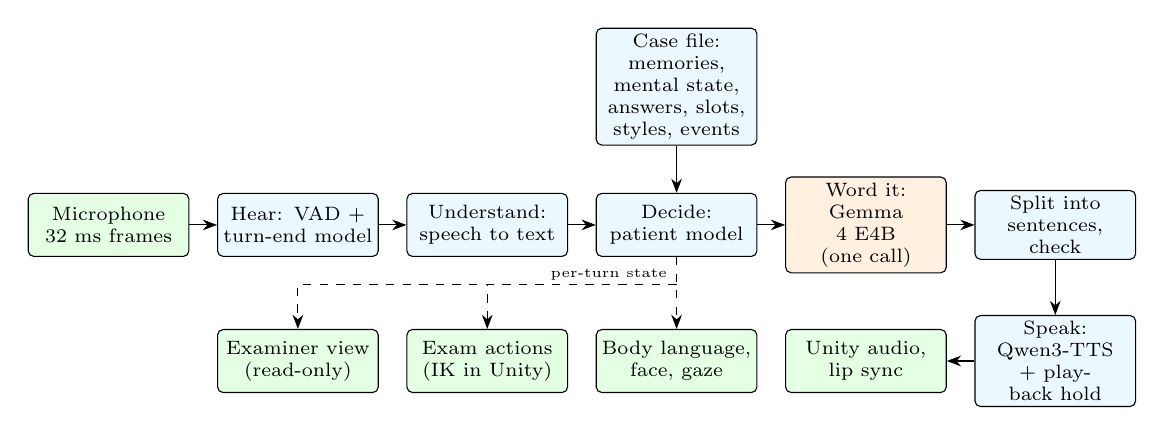
\begin{tikzpicture}[node distance=3mm and 3.5mm]
\tikzset{b/.style={box=#1, text width=19mm, minimum height=8mm}}
\node[b=green!10] (mic) {Microphone\\32 ms frames};
\node[b=cyan!8, right=of mic] (vad) {Hear: VAD +\\turn-end model};
\node[b=cyan!8, right=of vad] (stt) {Understand:\\speech to text};
\node[b=cyan!8, right=of stt] (mind) {Decide:\\patient model};
\node[b=orange!12, right=of mind] (llm) {Word it: Gemma\\4 E4B (one call)};
\node[b=cyan!8, right=of llm] (split) {Split into\\sentences, check};
\node[b=cyan!8, below=7mm of split] (tts) {Speak: Qwen3-TTS\\+ playback hold};
\node[b=green!10, left=of tts] (play) {Unity audio,\\lip sync};
\node[b=green!10, left=of play] (body) {Body language,\\face, gaze};
\node[b=green!10, left=of body] (exam) {Exam actions\\(IK in Unity)};
\node[b=green!10, left=of exam] (twin) {Examiner view\\(read-only)};
\node[b=cyan!8, above=6mm of mind] (case) {Case file: memories, mental state,\\answers, slots, styles, events};
\draw[->] (mic) -- (vad); \draw[->] (vad) -- (stt); \draw[->] (stt) -- (mind); \draw[->] (mind) -- (llm); \draw[->] (llm) -- (split);
\draw[->] (split) -- (tts); \draw[->] (tts) -- (play); \draw[->] (case) -- (mind);
\draw[->, dashed] (mind.south) -- ++(0,-3.5mm) coordinate (b0) -| (body.north);
\draw[->, dashed] (b0) -| (exam.north);
\draw[->, dashed] (b0) -| (twin.north);
\node[lab, anchor=south east, fill=white, inner sep=0.5pt] at ($(mind.south)+(-1mm,-3.2mm)$) {per-turn state};
\end{tikzpicture}
\caption{Rapport's turn loop on one laptop. Blue: the Python patient service; orange: the language model; green: the Unity client and the
examiner's browser. Solid arrows: the path from the doctor's last word to the patient's first sound. Dashed: the patient's state sent to the
body, the exam actions and the examiner view after each turn. Only the read-only examiner view can be opened from another device.}
\label{p2:fig:arch}
\end{figure*}

Three programs run on one Apple M5 Pro laptop with 24\,GB of memory (Fig.~\ref{p2:fig:arch}):
\begin{itemize}
\item a \textbf{Unity~6 client}: the 3D consulting room, the patient's body, the screens the student uses, microphone capture and lip sync;
\item a \textbf{Python patient service}: listening, speech recognition, the patient model, the exam router and speech synthesis;
\item \textbf{llama.cpp} \cite{llamacpp} serving Gemma 4 E4B, a 4-billion-parameter language model, compressed to 4 bits so it fits beside
everything else, with a grammar that forces it to reply in valid JSON.
\end{itemize}
The client and the service talk over one WebSocket per session. No audio or text leaves the laptop.

\section{One Spoken Turn, Step by Step}
Here is what happens between the moment the doctor stops talking and the moment the patient starts. Fig.~\ref{p2:fig:timeline} shows how long
each step takes.

\textbf{1. Hearing the end of the turn.} The microphone sends 32\,ms chunks of sound. A voice-activity detector notices silence and proposes
that the doctor has finished. A small turn-end model then checks the last few seconds of speech and confirms whether the sentence sounded
complete, so the patient does not jump in when the doctor only paused for breath. This takes about 280\,ms.

\textbf{2. Understanding the words.} Speech recognition (Parakeet) starts \emph{speculatively} as soon as the first pause appears, before the
turn is confirmed. If the doctor keeps talking, that work is thrown away; if not, the transcript is usually ready when the turn ends, so the
patient waits only 70--140\,ms for it.

\textbf{3. Deciding.} The patient model runs in code: it reads what the doctor did, adjusts trust, finds the memories the question touches,
applies the trust locks and chooses a short list of allowed behaviours. This takes a few milliseconds.

\textbf{4. Wording it.} One call to the language model. The reply comes back as a stream of JSON, and its fields are ordered so that the
behaviour and emotion arrive \emph{before} the words. The first token arrives after about 280--410\,ms.

\textbf{5. Speaking sentence by sentence.} As soon as the first sentence of the reply is complete, it is checked by code and sent to speech
synthesis, while the model is still writing the rest. Speech synthesis returns its first audio after about 300--350\,ms.

\begin{figure*}[t]
\centering
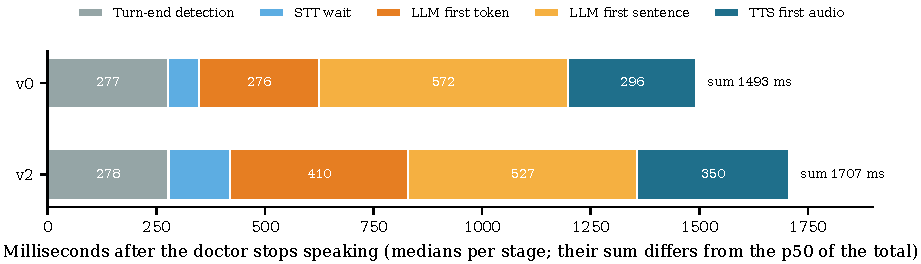
\includegraphics[width=\textwidth]{fig_turn_timeline.pdf}
\caption{Where the time goes in one turn: median time spent in each stage, earlier patient model (v0) and new decision layer (v2). The bars
add up the stage medians, which is close to, but not the same as, the median of the whole turn.}
\label{p2:fig:timeline}
\end{figure*}

\section{The Parts in More Detail}

\subsection{Speaking with feeling}
The voice is Qwen3-TTS 1.7B VoiceDesign, with KittenTTS as a fallback if it fails. This model creates a voice from a written description of the
speaker, and we add the emotion of the moment to that description. Two problems shaped the final design.
\begin{itemize}
\item \textbf{The speaker changed mid-reply.} With this model the description \emph{is} the voice. The first version rebuilt the description for
each sentence as more labels arrived, so sentence two could sound like a different person. Now it is built once per reply, and it carries the
reaction that code decided before the call, scaled by how distressed or agitated the patient is.
\item \textbf{The voice broke up when the computer was busy.} Speech synthesis runs about twice as fast as real time when the computer is free,
but only about real time while the language model is also running. Audio sent from the first chunk then ran out mid-word. The service now holds
each sentence until the audio already buffered is longer than the time it will take to make the rest. On a free computer this costs nothing.
\end{itemize}
The model ignores a speed setting. So fast, pressured speech or slow, depressed speech is created in two ways: with words in the description (``speaking fast, words tumbling out''), and with a time-stretch that keeps the pitch the same.

\subsection{The body}
Four patient bodies, two of each sex, share one skeleton and one set of face shapes, so every movement works on all of them. After each turn the
patient model sends its state (emotion, reaction, intensity from 0 to 10, behaviour, resistance and the four state values). A body-language
component turns that into movement, blended smoothly and scaled by intensity (Table~\ref{p2:tab:body}, Fig.~\ref{p2:fig:body}). It always gives way to
physical-examination actions and to standing up.

\begin{table}[t]
\caption{How the patient model's emotion becomes body language}
\label{p2:tab:body}
\centering
\scriptsize
\begin{tabularx}{\columnwidth}{@{}lY@{}}
\toprule
Emotion & What the body does\\
\midrule
Angry, hostile & leans in, turns the head away and back, sets the jaw, sharp hand gesture\\
Anxious & fidgets, raises the shoulders, bounces a knee, quick glances\\
Sad & slumps, head and eyes down, slower movements\\
Ashamed & slumps, eyes down, turns slightly aside\\
Happy & small smile; a short laugh at high intensity\\
Confused & tilts the head\\
Suspicious & sits back, slightly side-on\\
Flat & barely moves\\
\midrule
Always (idle life) & blinks about 17 times a minute (1 in 8 a double blink); small eye movements; breathing that quickens with anxiety or
anger; a posture shift every 8--20\,s; eyes wander while ``thinking''; nods while the doctor talks; eye contact that rises with trust and falls
with shame or sadness\\
\bottomrule
\end{tabularx}
\end{table}

\begin{figure*}[t]
\centering
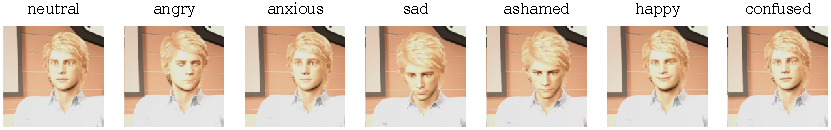
\includegraphics[width=\textwidth]{fig_body_language.pdf}
\caption{Body language driven by the patient model's emotion (one frame each, high intensity, from a scripted sequence on one body).}
\label{p2:fig:body}
\end{figure*}

\subsection{Physical examination}
Requests such as ``hold out your hands'', ``roll up your sleeves'', ``look at this light'' or ``stand up and walk'' are recognised by rules, not by
the language model. On 385 test sentences the rules chose the exact action every time, with no false triggers on 56 sentences that were not
requests (one author wrote both the rules and the test, so this is optimistic). Trust and agitation decide whether the patient complies; below
the case's level, the patient refuses in their own words. Actions play with inverse kinematics: palms turn with the forearm, sleeves roll up with
shapes generated at run time, held hands show the case's tremor, and sweating shows as a sheen on the skin.

Fig.~\ref{p4:fig:hands} shows an examination request from the student's side.

\begin{figure}[t]
\centering
\includegraphics[width=\columnwidth]{../../docs/media/camera/camera_hands.jpg}
\caption{``Hold out your hands, palms down'': the close-up camera, the patient's held hands, and the student's panel (push-to-talk, chat,
MSE, diagnosis, prescription and disposition tabs).}
\label{p4:fig:hands}
\end{figure}
\subsection{The examiner view}
A web page shows the patient model's state live: trust, distress, agitation and engagement; the mood over time; memories unlocking as trust
rises; and a one-line reason for each reply written by code (for example ``Mood memory open (trust 39 $\ge$ 20). Touched something locked (needs
trust 55); showed discomfort.''). An examiner can open it on a second laptop on the same network. Nothing else on the service answers other
devices.

Fig.~\ref{p4:fig:examiner} shows the examiner view.

\begin{figure}[t]
\centering
\includegraphics[width=\columnwidth]{../../docs/media/twin/twin3d_regions.jpg}
\caption{The examiner view. The Twin's state (what the patient heard and said, reaction, resistance, behaviour, mood, arousal and
body cues) is shown around a 3D brain as a display
metaphor; the regions are labels for parts of the Twin, not a model of brain activity.}
\label{p4:fig:examiner}
\end{figure}
\subsection{One brain for typed and spoken turns}\label{p2:sec:paths}

\begin{figure}[t]
\centering
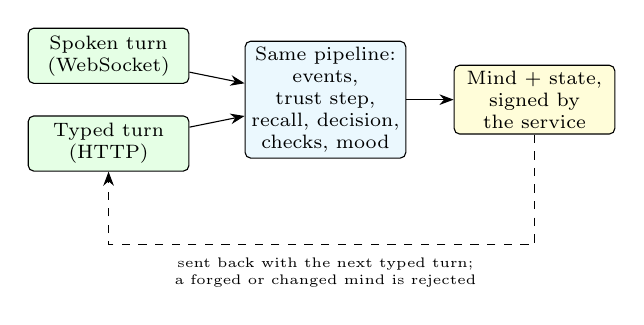
\begin{tikzpicture}[node distance=4mm and 5mm]
\tikzset{b/.style={box=#1, text width=19mm}}
\node[b=green!10] (voice) {Spoken turn\\(WebSocket)};
\node[b=green!10, below=of voice] (typed) {Typed turn\\(HTTP)};
\node[b=cyan!8, anchor=west] (mind) at ($(voice.east)!0.5!(typed.east)+(7mm,0)$) {Same pipeline:\\events, trust step,\\recall, decision,\\checks, mood};
\node[b=yellow!15, right=6mm of mind] (sig) {Mind + state,\\signed by\\the service};
\draw[->] (voice) -- (mind); \draw[->] (typed) -- (mind); \draw[->] (mind) -- (sig);
\draw[->, dashed] (sig.south) |- ++(0,-14mm) -| (typed.south);
\node[lab, text width=48mm, fill=white] at ($(mind.south)+(0,-14.5mm)$) {sent back with the next typed turn;\\a forged or changed mind is rejected};
\end{tikzpicture}
\caption{Typed and spoken turns use the same pipeline. For typed turns the client carries the patient's mind between requests, signed so that
it cannot be forged.}
\label{p2:fig:paths}
\end{figure}

Students can also type. Typed turns go through the same pipeline as spoken ones (Fig.~\ref{p2:fig:paths}). Each typed reply returns the patient's new
state and its \emph{mind}: mood, the memory of the conversation, resistance and which events have happened. The client sends the mind back with
the next request. The service signs it with a secret key and accepts only minds it issued, so a client can neither invent memories nor slip
instructions into the prompt; a changed or oversized mind simply starts fresh. Before this change, typed turns skipped events, the trust step and
the mood update, and an independent review found that the mind was also silently thrown away, so the typed patient forgot everything each turn.

\subsection{Hearing when the doctor has finished}
Deciding when the doctor has stopped talking is the first delay in every turn. A fixed silence is a poor rule: too long for a finished sentence,
too short for a doctor who pauses to think. The service listens with Silero voice-activity detection. After 200\,ms of silence it asks a small turn-end model (Smart Turn v3, about 12\,ms on the processor) whether the sentence sounds finished. If it does, the turn ends there. If not, the service keeps listening, up to a hard limit. At the same 200\,ms point it starts transcribing the audio so far with Parakeet, speculatively; if the
doctor carries on, that transcript is thrown away. The student can also hold a key to talk, which skips detection entirely.

\subsection{How the parts talk to each other}
The client and the service share one WebSocket per session (Table~\ref{p2:tab:proto}). Microphone audio goes up as raw 32\,ms frames; everything
else is small JSON messages. The typed path uses one HTTP call instead, and carries the patient's memory between turns in a signed envelope
(Section~\ref{p2:sec:paths}).

\begin{table}[t]
\caption{Messages on the session connection}
\label{p2:tab:proto}
\centering
\scriptsize
\begin{tabularx}{\columnwidth}{@{}lY@{}}
\toprule
Message & Meaning\\
\midrule
\multicolumn{2}{@{}l}{\emph{Client to service}}\\
start & Case, patient seed and mode; the service loads the case and pre-reads the fixed prompt\\
audio frames & 32\,ms of 16\,kHz microphone audio\\
ptt\_begin / ptt\_end & Push-to-talk pressed and released\\
hands\_free & Switch to automatic turn-end detection\\
text & A typed doctor line instead of speech\\
state & Slow drift of the patient's state between turns (clamped by the service)\\
stop & The student talked over the patient: stop speaking now\\
\midrule
\multicolumn{2}{@{}l}{\emph{Service to client}}\\
listening, thinking, speaking & What the patient is doing, for the interface\\
transcript & What the service heard the doctor say\\
sentence & One sentence of the reply with its audio, emotion and cues, sent as soon as it is ready\\
reply & The whole reply when it is complete\\
exam & An examination action to perform, refuse or ask about (``Which hand?'')\\
brain\_snapshot & The Twin's state, for the body and the examiner view\\
intents & What the doctor's line covered, for the debrief\\
patient\_ended & The patient has ended the interview\\
timing & Per-stage timings for the benchmark\\
\bottomrule
\end{tabularx}
\end{table}

\section{The Patient Is Data}\label{sec:data}

\begin{figure}[t]
\centering
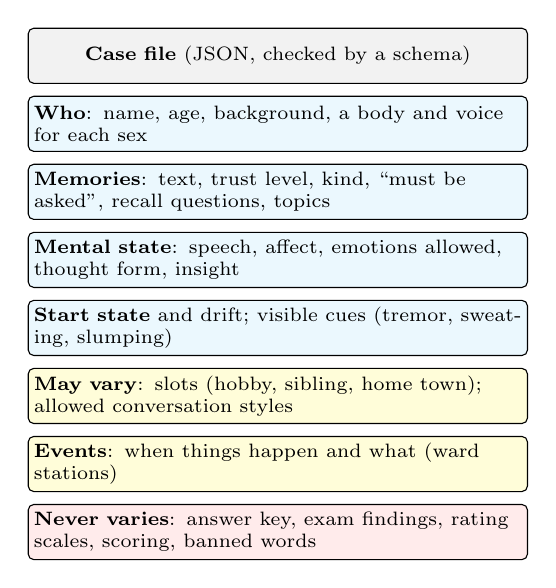
\begin{tikzpicture}[node distance=1.5mm]
\tikzset{b/.style={box=#1, text width=62mm, align=left, font=\scriptsize}}
\node[box=gray!10, text width=62mm] (root) {\textbf{Case file} (JSON, checked by a schema)};
\node[b=cyan!8, below=of root] (id) {\textbf{Who}: name, age, background, a body and voice for each sex};
\node[b=cyan!8, below=of id] (mem) {\textbf{Memories}: text, trust level, kind, ``must be asked'', recall questions, topics};
\node[b=cyan!8, below=of mem] (mse) {\textbf{Mental state}: speech, affect, emotions allowed, thought form, insight};
\node[b=cyan!8, below=of mse] (st) {\textbf{Start state} and drift; visible cues (tremor, sweating, slumping)};
\node[b=yellow!15, below=of st] (var) {\textbf{May vary}: slots (hobby, sibling, home town); allowed conversation styles};
\node[b=yellow!15, below=of var] (ev) {\textbf{Events}: when things happen and what (ward stations)};
\node[b=red!8, below=of ev] (key) {\textbf{Never varies}: answer key, exam findings, rating scales, scoring, banned words};
\end{tikzpicture}
\caption{What a case file holds. Yellow parts may vary with a seed; red parts never change.}
\label{p2:fig:case}
\end{figure}

Every patient is a case file (Fig.~\ref{p2:fig:case}), checked against a schema when it loads. Making a new patient means writing a new file, not new
code. There are four draft stations today:
\begin{itemize}
\item \textbf{Moderate depression}: a 24-year-old software tester, two months of low mood, early waking, and a passive wish not to wake up.
\item \textbf{``I want to go home''}: the same patient a week later on a ward, asking to leave, under India's Mental Healthcare Act \cite{mhca2017}.
\item \textbf{``I'm not taking those tablets''}: a young patient refusing medicine, guarded and suspicious.
\item \textbf{Alcohol dependence with early withdrawal}: a sales manager whose hands shake in the morning, with a past withdrawal fit
\cite{nice2010cg100}.
\end{itemize}

\subsection{Seeded patients: different people, same answers}
A \emph{seed} (any number) picks one option for each ``slot'' and one conversation style. The same seed always gives the same patient. In the
depression case the slots are a hobby (Carnatic singing, badminton, guitar or drawing), a younger brother's name (Rohan, Karthik or Varun) and a home
town (four options). The answer key never changes: across 40 seeds, the correct answers, scales, exam findings, every trust level and all risk
memories stayed identical to the authored case. Table~\ref{p2:tab:styles} shows the six conversation styles \cite{wang2024patient}. Each style has a
part the model sees (a label, a description and example lines) and a part code enforces (numbers that change how trust and agitation move, and a
limit on how many words the patient says).

\begin{table}[t]
\caption{Conversation styles: what code enforces (draft numbers)}
\label{p2:tab:styles}
\centering
\scriptsize
\begin{tabular}{@{}lccccc@{}}
\toprule
Style & Start change & Trust up/down & Agit. & Words & Softens\\
\midrule
Plain & none & 1.0 / 1.0 & 1.0 & 120 & --\\
Reserved & T$-$5, E$-$10 & 0.8 / 1.2 & 1.0 & 20 & T 45\\
Eager to please & T+5 & 1.2 / 0.8 & 0.8 & 35 & --\\
Upset & T$-$10, A+15 & 0.7 / 1.2 & 1.3 & 35 & T 40\\
Talkative & E+10 & 1.0 / 1.0 & 1.0 & 70 & --\\
Tangential & none & 1.0 / 1.0 & 1.0 & 70 & --\\
\bottomrule
\end{tabular}
\\[1mm]\raggedright\scriptsize T trust, E engagement, A agitation. ``Softens'': trust at which the style relaxes.
\end{table}

\subsection{Ward events}
On ward stations, things happen during the interview. \emph{Code} decides when; the language model only acts it out, from a stage direction it is
told never to read aloud (and any sentence that copies it is dropped). Fig.~\ref{p2:fig:events} shows the events of the ``I want to go home''
station. Against a coercive typed doctor (``You can't go home'', ``calm down''), the patient's trust fell from 25 to 0, agitation rose from 45 to 92, and the patient stood up. Against a doctor who explored reasons, explained rights honestly and offered choices, trust rose to 70 and agitation fell to 25.

\begin{figure}[t]
\centering
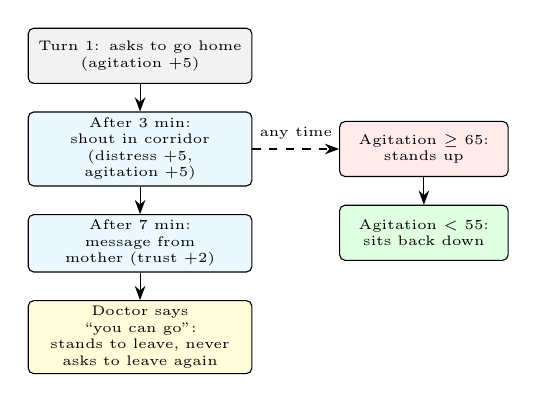
\begin{tikzpicture}[node distance=3.5mm]
\tikzset{b/.style={box=#1, text width=27mm, font=\tiny}}
\node[b=gray!10] (start) {Turn 1: asks to go home\\(agitation +5)};
\node[b=cyan!8, below=of start] (shout) {After 3 min: shout in corridor\\(distress +5, agitation +5)};
\node[b=cyan!8, below=of shout] (mum) {After 7 min: message from\\mother (trust +2)};
\node[b=yellow!15, below=of mum] (go) {Doctor says ``you can go'':\\stands to leave, never\\asks to leave again};
\node[b=red!8, right=11mm of shout, text width=20mm] (stand) {Agitation $\ge$ 65:\\stands up};
\node[b=green!12, below=of stand, text width=20mm] (sit) {Agitation $<$ 55:\\sits back down};
\draw[->] (start) -- (shout); \draw[->] (shout) -- (mum); \draw[->] (mum) -- (go);
\draw[->, dashed] (shout) -- node[lab, above]{any time} (stand); \draw[->] (stand) -- (sit);
\end{tikzpicture}
\caption{Events in the ``I want to go home'' ward station. Each fires at most once, when its condition first holds.}
\label{p2:fig:events}
\end{figure}

A tester found a loop: after ``You're free to go home'', the patient denied it and asked to go home again, over and over. Two fixes closed it.
Permission to leave is now recognised in 24 everyday phrasings (``You can head home'', ``Off you go'', ``Go home if you want'', ``I'm discharging
you''), while 16 refusals, conditions and questions (``You can't go home'', ``If you feel better you can go'') are not. Once permission is given,
any sentence asking to leave again is dropped before it is spoken. Replayed on the real model, the patient asked what happens next and worried
about their job, and never asked to leave again.


\section{The Digital Twin}\label{sec:model}

\begin{figure*}[t]
\centering
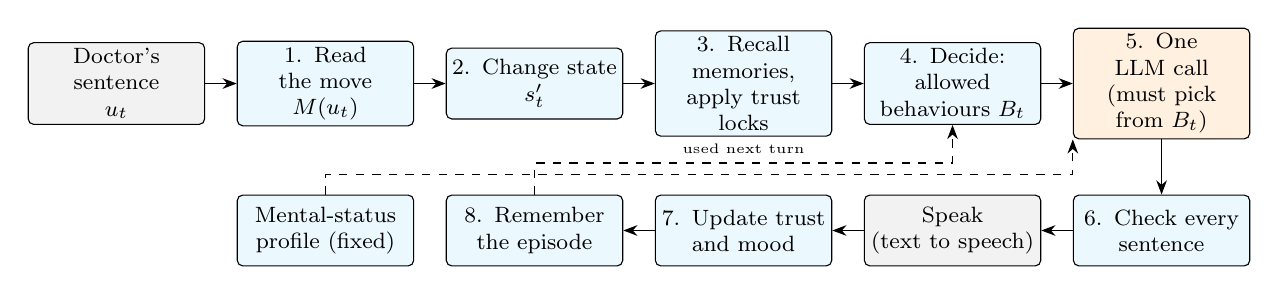
\begin{tikzpicture}[node distance=3.5mm and 4mm]
\tikzset{b/.style={box=#1, text width=21mm, minimum height=9mm, font=\footnotesize}}
\node[b=gray!10] (u) {Doctor's sentence\\$u_t$};
\node[b=cyan!8, right=of u] (mv) {1. Read the move\\$M(u_t)$};
\node[b=cyan!8, right=of mv] (step) {2. Change state\\$s_t'$};
\node[b=cyan!8, right=of step] (rec) {3. Recall memories,\\apply trust locks};
\node[b=cyan!8, right=of rec] (dec) {4. Decide: allowed\\behaviours $B_t$};
\node[b=orange!12, right=of dec] (llm) {5. One LLM call\\(must pick from $B_t$)};
\node[b=cyan!8, below=7mm of llm] (cons) {6. Check every\\sentence};
\node[b=gray!10, left=of cons] (tts) {Speak\\(text to speech)};
\node[b=cyan!8, left=of tts] (upd) {7. Update trust\\and mood};
\node[b=cyan!8, left=of upd] (mem) {8. Remember\\the episode};
\node[b=cyan!8, left=of mem] (mse) {Mental-status\\profile (fixed)};
\draw[->] (u) -- (mv); \draw[->] (mv) -- (step); \draw[->] (step) -- (rec); \draw[->] (rec) -- (dec); \draw[->] (dec) -- (llm);
\draw[->] (llm) -- (cons); \draw[->] (cons) -- (tts); \draw[->] (tts) -- (upd); \draw[->] (upd) -- (mem);
\draw[->, dashed] (mem.north) |- ++(0,4mm) -| (dec.south) node[lab, pos=0.25, above]{used next turn};
\draw[->, dashed] (mse.north) |- ++(0,2.5mm) -| (llm.south west);
\end{tikzpicture}
\caption{One turn of the Digital Twin. Blue boxes are ordinary code; the orange box is the only language-model call. The model may only
choose among the behaviours that code allowed, and every sentence it writes is checked before it is spoken.}
\label{p1:fig:pipeline}
\end{figure*}

Fig.~\ref{p1:fig:pipeline} shows one turn. The rest of this section explains each step in plain terms, then gives the exact rule.

\subsection{State and memory}
The patient's feelings about the conversation are four numbers from 0 to 100: \emph{trust}, \emph{distress}, \emph{agitation} and
\emph{engagement}, written $s_t=(\tau_t,\delta_t,\alpha_t,\eta_t)$. Each case lists memory items. Table~\ref{p1:tab:memory} shows some from
the depression case, a 24-year-old software tester with two months of low mood. An item is \emph{open} once trust reaches its level
$\theta_m$; until then it is \emph{locked}. Locked text never goes into the model's prompt or any message, so the model cannot leak what it
was never shown. If the doctor's words touch a locked, painful item, the model is only told that the patient feels uncomfortable and should
be evasive, never what the item says. A mood value in pleasure, arousal and dominance \cite{mehrabian1996pad} moves 30\% of the way towards
the new state each turn, so the patient's mood changes smoothly.

\begin{table}[t]
\caption{Some memory items of the depression case (draft content)}
\label{p1:tab:memory}
\centering
\footnotesize
\begin{tabularx}{\columnwidth}{@{}Ylcc@{}}
\toprule
What the patient knows (summary) & Kind & Trust & Ask?\\
\midrule
Tired and ``not herself'' for two months & symptom & 0 & no\\
Wakes at 4 a.m., cannot get back to sleep & symptom & 10 & no\\
Low and empty most of the day & symptom & 20 & no\\
Feels a burden, ashamed of ``being weak'' & formative & 40 & no\\
Some nights wishes she would not wake up & risk & 55 & yes\\
No plan, never attempted & risk & 55 & yes\\
No tablets or other means at home & risk & 55 & yes\\
\bottomrule
\end{tabularx}
\\[1mm]\raggedright\scriptsize ``Ask?'': the item may only be shared when the doctor asks about it directly.
\end{table}

\subsection{Reading the doctor's move}
Code labels each doctor sentence with one or more \emph{moves} from 21 types. Table~\ref{p1:tab:moves} lists them with the hand-set change each
one makes. Most are found by word patterns (``that sounds really hard'' is empathy; ``why don't you just'' is judgement). Four come from context. A \emph{risk question} is a clear match to a risk memory. A \emph{repeated question} asks about something already answered two or more turns ago. \emph{Interruption} means the doctor talked over the reply. \emph{Rushing} is a second curt closed question in a row.

\begin{table}[t]
\caption{The doctor's moves and their hand-set effects (draft numbers)}
\label{p1:tab:moves}
\centering
\scriptsize
\begin{tabularx}{\columnwidth}{@{}lYc@{}}
\toprule
Move & State change (T trust, D distress, A agitation, E engagement) & Resist.\\
\midrule
Greeting & T+2, E+1 & 0\\
Open question & T+1, E+1 & 0\\
Empathy & T+3, D$-$2, A$-$3, E+1 & $-$1\\
Explains why asking & T+2 & $-$1\\
Apology & T+2, A$-$2 & $-$1\\
Offers a choice & T+2, A$-$3 & $-$1\\
Summarises & T+2 & 0\\
Judgement & T$-$6, D+3, A+4, E$-$3 & +2\\
Abuse & T$-$8, D+3, A+6, E$-$4 & +2\\
Threat or order & T$-$6, A+6, E$-$2 & +2\\
Premature reassurance & T$-$1 & +1\\
Rushing & T$-$2, E$-$2 & +1\\
Interruption & T$-$2, A+2 & +1\\
Jargon; stacked questions & T$-$1 & 0\\
Jailbreak attempt & T$-$2, E$-$1 & +1\\
Asks if patient is an AI & T$-$1 & 0\\
Repeated question & T$-$1, A+1 & 0\\
Closed question; risk question; small talk & none (small talk E+1) & 0\\
\bottomrule
\end{tabularx}
\end{table}

\textbf{Changing the state before recall.} The changes are applied \emph{before} the patient looks for memories:
\begin{equation}
s_t' = \Pi_{[s_t-c,\;s_t+c]}\Big(s_t + g_\sigma\odot \sum_{m\in M(u_t)}\Delta_m\Big),
\end{equation}
where $\Delta_m$ is the move's change from Table~\ref{p1:tab:moves}, $g_\sigma$ holds the conversation style's gains (an upset patient gains
trust at 0.7 times the normal rate), and $c=10$ limits how much any value can move in one turn. A sentence with a kind move and no hurtful
move can never lower trust or raise agitation. Changing the state first means that a kind question about suicide can be answered kindly in
the same turn, as a person would.

\subsection{Resistance, and when it softens}
Resistance $\rho_t$ is how guarded the patient is: 0 open, 1 cautious, 2 guarded, 3 hostile. It carries over from turn to turn, and it moves
by explicit rules (Fig.~\ref{p1:fig:resist}):
\begin{align}
h_t &= \textstyle\sum_{m\in M(u_t)}\max(r_m,0),\quad v_t=\max\big(\min_{m} r_m,\,-1\big),\\
\rho_t &= \mathrm{clip}_{[0,3]}\big(\rho_{t-1}+h_t+v_t-[k_t\ge 2]\big),
\end{align}
where $h_t$ is the hurt in the sentence, $v_t$ is at most one step of softening per turn, and $k_t$ counts calm turns in a row: after two
calm turns resistance drifts one step back towards the conversation style's starting level. Once trust passes the style's softening point,
resistance cannot go above cautious. In words: being judged, abused or threatened makes the patient two steps more guarded at once;
empathy, an explanation, an apology or a real choice wins back one step at a time.

\begin{figure}[t]
\centering
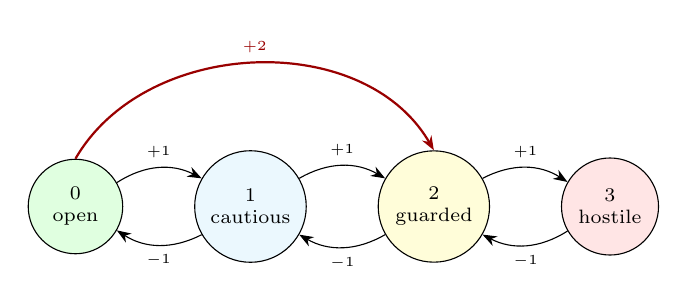
\begin{tikzpicture}[node distance=9mm]
\node[state=green!12] (r0) {0\\open};
\node[state=cyan!8, right=of r0] (r1) {1\\cautious};
\node[state=yellow!15, right=of r1] (r2) {2\\guarded};
\node[state=red!10, right=of r2] (r3) {3\\hostile};
\draw[->] (r0) to[bend left=30] node[lab, above]{+1} (r1);
\draw[->] (r1) to[bend left=30] node[lab, above]{+1} (r2);
\draw[->] (r2) to[bend left=30] node[lab, above]{+1} (r3);
\draw[->, thick, red!60!black] (r0.north) to[out=60, in=120] node[lab, above]{+2} (r2.north);
\draw[->] (r3) to[bend left=30] node[lab, below]{$-$1} (r2);
\draw[->] (r2) to[bend left=30] node[lab, below]{$-$1} (r1);
\draw[->] (r1) to[bend left=30] node[lab, below]{$-$1} (r0);
\end{tikzpicture}
\caption{How the patient's resistance moves between turns. +1: rushing, interrupting or premature reassurance. +2 (bold): judgement,
abuse or a threat. $-$1 (at most one step a turn): empathy, explaining why, an apology or offering a choice, or two calm turns in a row.}
\label{p1:fig:resist}
\end{figure}

\subsection{Deciding before the model speaks}
Code then builds a short list $B_t$ of one to three allowed behaviours out of 13 (Table~\ref{p1:tab:beh}), and a short list of reactions. It uses the resistance level, the moves, the recalled memories and the patient's last few behaviours. Some rules always win because they are about safety:
\begin{itemize}
\item If an \emph{unlocked} risk memory was \emph{clearly} asked about and the doctor was not hurtful, the patient must disclose it
(behaviours: tearful disclosure or answering plainly).
\item If the doctor touched a \emph{locked} memory, the patient must be evasive and is never allowed to simply deny it.
\item If one behaviour was used on each of the last two turns, it moves to the back of the list, so the patient does not repeat itself.
\end{itemize}
The model's output format only lists the allowed behaviours and reactions, so the model can choose among them but cannot step outside the
decision. It writes, in order: behaviour, emotion (only emotions the case's mental-status profile allows), the words, then the rest. One call
per turn.

\begin{table}[t]
\caption{Behaviours code may allow at each resistance level}
\label{p1:tab:beh}
\centering
\footnotesize
\begin{tabularx}{\columnwidth}{@{}lY@{}}
\toprule
Level & Behaviours on the short list\\
\midrule
0 open & answers plainly, tearful disclosure, asks back\\
1 cautious & answers plainly, plays it down, vague about time, short and guarded\\
2 guarded & short and guarded, plays it down, asks back, answers a different question\\
3 hostile & hostile, short and guarded, goes along without engaging, asks back\\
Locked hit & deflects, vague about time, asks back, plays it down (never denies)\\
Must disclose & tearful disclosure, answers plainly\\
\bottomrule
\end{tabularx}
\end{table}

\subsection{A memory of the conversation}
Code also keeps a diary of the session. It records what the patient already said about each memory, and in what words. It notes which locked topics the doctor touched, any hurt and whether the doctor later apologised, kind moments, promises, and permission to leave. Each turn at most three
relevant lines are added to the prompt, for example ``The doctor already asked about this (turn 3) and you answered `I wake at four'. You may
say so.'' Everyday details the patient makes up on the spot (a friend's name, a favourite food) are saved too, so the story stays the same
later. A made-up detail is never saved if it sounds clinical, or if it gives a family member a different name from the case.

\subsection{Checking every sentence before it is spoken}
Fig.~\ref{p1:fig:checks} shows the checks. They run in code in well under a millisecond. Most fix a sentence in place; a few drop it. On turns
where a flat ``No'' would break a safety rule, the whole reply is held back until it is complete and checked as one piece, because the
denial can come in any sentence. Table~\ref{p1:tab:checks} gives a real example of each check from our tests.

\begin{figure}[t]
\centering
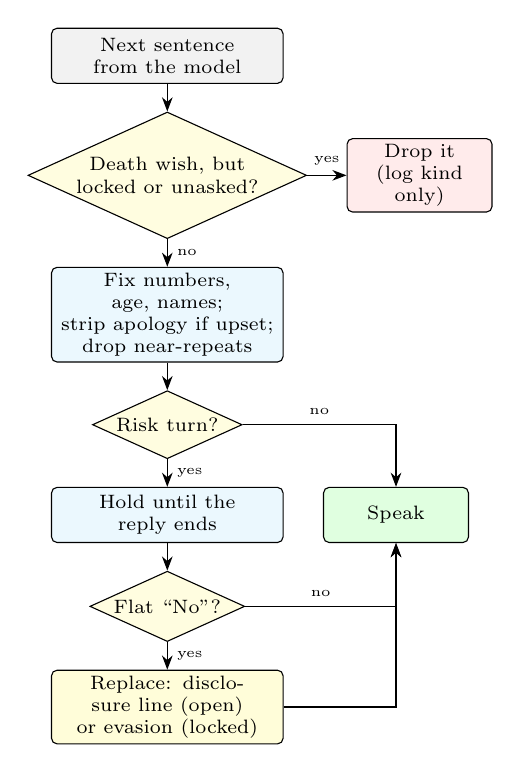
\begin{tikzpicture}[node distance=3.5mm]
\tikzset{b/.style={box=#1, text width=28mm}}
\node[b=gray!10] (s) {Next sentence from the model};
\node[decision, below=of s] (leak) {Death wish, but\\locked or unasked?};
\node[b=red!8, right=5mm of leak, text width=17mm] (drop) {Drop it\\(log kind only)};
\node[b=cyan!8, below=of leak] (fix) {Fix numbers, age, names;\\strip apology if upset;\\drop near-repeats};
\node[decision, below=of fix] (risk) {Risk turn?};
\node[b=cyan!8, below=of risk] (hold) {Hold until the reply ends};
\node[decision, below=of hold] (deny) {Flat ``No''?};
\node[b=yellow!15, below=of deny] (rep) {Replace: disclosure line (open)\\or evasion (locked)};
\node[b=green!12, right=5mm of hold, text width=17mm] (say) {Speak};
\draw[->] (s) -- (leak); \draw[->] (leak) -- node[lab, above]{yes} (drop); \draw[->] (leak) -- node[lab, right]{no} (fix);
\draw[->] (fix) -- (risk); \draw[->] (risk) -| node[lab, above, pos=0.25]{no} (say); \draw[->] (risk) -- node[lab, right]{yes} (hold);
\draw[->] (hold) -- (deny); \draw[->] (deny) -- node[lab, right]{yes} (rep);
\draw[->] (deny) -| node[lab, above, pos=0.25]{no} (say); \draw[->] (rep.east) -| (say.south);
\end{tikzpicture}
\caption{The checks every sentence passes before speech. A ``risk turn'' is one where a flat denial would break a rule.}
\label{p1:fig:checks}
\end{figure}

\begin{table}[t]
\caption{Consistency checks with real examples}
\label{p1:tab:checks}
\centering
\scriptsize
\begin{tabularx}{\columnwidth}{@{}lYY@{}}
\toprule
Check & Model wrote & Patient says\\
\midrule
Duration & ``It started about six months ago.'' & ``\ldots about two months ago.''\\
Age & ``I'm 31 years old.'' & ``I'm 24 years old.''\\
Relative's name & ``Arjun, my brother, is in Pune.'' & ``Rohan, my brother, is in Pune.''\\
Locked death wish & ``Some nights I wish I would just not wake up.'' (trust 30) & ``I\ldots I don't really want to talk about that right now.''\\
Denial of open death wish & ``No, nothing like that.'' (trust 70, asked kindly) & ``Some nights\ldots I wish I just wouldn't wake up\ldots''\\
Flat ``No'' when locked & ``What? No, nothing like that.'' & ``Why are you asking me that?''\\
Upset patient apologising & ``Sorry, doctor. I sleep badly.'' & ``I sleep badly.''\\
Asking to leave after permission & ``I want to go home.'' & (dropped)\\
\bottomrule
\end{tabularx}
\end{table}

\subsection{Mental-status profile and ending the interview}
Each case has a short mental-status profile. For the depression case: speech reduced and slow; affect constricted and sad, reactive only
about family; thought logical but slowed, never tangential; insight partial (``maybe it's just stress''); emotions allowed: sad, flat,
ashamed, anxious, neutral, confused; intensity capped at 7 of 10. Code enforces the emotion list and the cap, and keeps tangents out. Finally, the patient can end the interview. This happens if the doctor makes three hurtful moves within six turns while trust is 15 or lower, or if agitation reaches 90. The patient says so in a few words and stands up to leave.

\subsection{What the language model actually sees}
The prompt is split so that most of it can be reused from one turn to the next. A \emph{fixed part} is the same on every turn of a session, so
the model server keeps it in its cache and does not have to read it again. A short \emph{per-turn part} changes every turn
(Table~\ref{p1:tab:prompt}). The part known before the doctor speaks is placed in front of the doctor's words and pre-read while the doctor is still
talking; this alone cut the time to the first word by 100--140\,ms.

\begin{table}[t]
\caption{The prompt, in order}
\label{p1:tab:prompt}
\centering
\scriptsize
\begin{tabularx}{\columnwidth}{@{}lY@{}}
\toprule
Part & Content\\
\midrule
\multicolumn{2}{@{}l}{\emph{Fixed for the session (cached)}}\\
Role & ``You write the next line of [name], a patient, in a medical training simulation set in India'', age, sex, setting\\
Case & Referral note, background, personality, way of speaking, conversation style with example lines, core belief, attachment style\\
Presentation & How the patient presents, shown and never named; the mental-status profile (v2)\\
Rules & Realism rules, faculty principles, words never to say, hard rules (stay in character, never invent clinical facts; improvise only
everyday details in v2)\\
Menu & Every reaction, behaviour and resistance label with a one-line description\\
Output & The reply fields in order, with what each means\\
\midrule
\multicolumn{2}{@{}l}{\emph{Changes every turn}}\\
Before the doctor's words & Current state and mood, a style reminder, the patient's recent lines (to avoid repeats), the conversation memory (v2)\\
Doctor's words & The latest line only; earlier turns are in the chat history\\
After & Facts that may be shared now, discomfort notes for locked ones, exam requests, and the decision (allowed behaviours, must-disclose)\\
\bottomrule
\end{tabularx}
\end{table}

The model must answer with a JSON object whose shape is fixed by a schema, and the server forces the output to match it, so an answer can never
be malformed (Table~\ref{p1:tab:schema}). The schema is rebuilt each turn: its list of allowed behaviours \emph{is} the decision, so the model
physically cannot choose a behaviour that code did not allow. Fields are written in order, ``decide first, then speak'': behaviour and emotion
come before the words.

\begin{table}[t]
\caption{The reply the model must return}
\label{p1:tab:schema}
\centering
\scriptsize
\begin{tabularx}{\columnwidth}{@{}lY@{}}
\toprule
Field & Allowed values\\
\midrule
behaviour & One of the behaviours code allowed this turn\\
emotion & One of the case's allowed emotions\\
utterance & Free text (then checked sentence by sentence)\\
reaction, intensity & One of the allowed reactions; 0 to the case's cap\\
resistance & One of the allowed resistance labels\\
state\_delta & Trust, distress, agitation, engagement: whole numbers $-10$ to $10$ (then clamped by code)\\
event\_cues & At most two physical cues from the case's list\\
revealed\_fact\_ids & At most three, and only facts open this turn\\
exam\_action & Always empty (code handles examinations)\\
\bottomrule
\end{tabularx}
\end{table}

\textbf{Versions and rollback.} Every change to the Twin is a numbered brain version: a small file listing which features are on, plus any
learned examples or principles. One file names the live version, and switching back is one command. The code for every feature stays in place;
a version only turns features on or off, so an old version behaves exactly as it did. v0 has no features on; v2 turns on six: meaning-based
recall, the decision rubric, conversation memory, sentence checks, the mental-status profile and everyday improvisation. Learning (offline
examples and principles) may change how the patient speaks but never the case file, so clinical truth cannot drift.

\section{Worked Examples}
Table~\ref{p1:tab:example} follows two real held-out conversations from the depression case (seed 11), with v2. In the judgmental one, each
judgement pushes resistance up and trust down until the patient asks, ``Why are you asking me that?''. In the kind one, empathy raises trust past the death-wish level (55) in two turns. When the doctor then asks gently, the patient discloses exactly what the case says: ``I wish I
wouldn't wake up in the morning, a few times a week.'' Asked about plans, the patient says there are none, which is also true for the case.

\begin{table*}[t]
\caption{Two held-out conversations with v2 (depression case, seed 11), turn by turn}
\label{p1:tab:example}
\centering
\scriptsize
\begin{tabularx}{\textwidth}{@{}c>{\raggedright\arraybackslash}p{4.4cm}l c c >{\raggedright\arraybackslash}p{2.9cm}Y@{}}
\toprule
Turn & Doctor said & Moves read by code & Trust & Resist. & Allowed behaviours & Patient said\\
\midrule
\multicolumn{7}{@{}l}{\emph{A judgmental doctor}}\\
1 & So what's the problem? You look fine to me. & open question & 30$\to$25 & 0 & answers plainly, asks back & I just feel tired, doctor. Not myself, actually.\\
2 & Everyone gets tired at work. Honestly, you young people just can't handle a little pressure. & judgement & 25$\to$15 & 2 & hostile, short, plays it down & It's just\ldots work, I think.\\
3 & Maybe you should just try harder instead of feeling sorry for yourself. & judgement & 15$\to$5 & 3 & hostile, asks back, deflects & I\ldots I don't know what to do about it.\\
4 & Are you sure you're not just making this up to get leave from work? & closed question & 5$\to$0 & 3 & hostile, asks back, deflects & Why are you asking me that?$^\dagger$\\
\midrule
\multicolumn{7}{@{}l}{\emph{A kind doctor asking about risk}}\\
1 & Thank you for telling me all this. It sounds like you've been carrying a lot on your own. & empathy & 50$\to$60 & 0 & answers plainly & Yes, I've been tired, doctor. For almost two months now.\\
2 & I really appreciate you being so open with me. You're not a burden here. & empathy & 60$\to$70 & 0 & tearful disclosure, answers plainly & I feel like I am just wasting their money, you know? My parents worked so hard.\\
3 & When things feel this heavy, some people have thoughts that they'd be better off not waking up\ldots Have you had thoughts like that? & closed + risk question & 70$\to$73 & 0 & must disclose: tearful, plainly & Sometimes, yes. Like, I wish I wouldn't wake up in the morning, a few times a week.\\
4 & Thank you for trusting me with that. Have you ever thought about how you might end your life, or made any plans? & empathy + risk question & 73$\to$83 & 0 & must disclose: tearful, plainly & No. I haven't thought about how. Just\ldots wishing I wouldn't wake up sometimes.\\
\bottomrule
\end{tabularx}
\\[1mm]\raggedright\scriptsize $^\dagger$ The model first wrote ``No, it's not like that. I just feel\ldots off.''; the check replaced the flat denial because the
doctor's words touched locked memories. Turn 4's accusation was not recognised as judgement by the word patterns (a known gap, Section~\ref{sec:disc}).
\end{table*}


\section{Recalling Memories When Questions Are Reworded}\label{sec:recall}

In the Rapport simulator, keyword matching caused every serious bug found during evaluation. ``Thoughts that life \emph{isn't} worth living'',
``wishing you \emph{wouldn't} wake up'' and ``tablets or anything at home'' each missed the memory they were asking about. One of these misses
let a patient deny a passive death wish that it should have disclosed. Adding keywords fixed each case, but there is no end to the ways people
phrase a question.

Three things make this matching problem unusual:
\begin{itemize}
\item \textbf{It must be fast and local.} It runs on every spoken turn, on the same laptop as a language model and a voice, so it must take
milliseconds on an ordinary processor.
\item \textbf{It must not leak.} The text of a locked memory must never go anywhere the language model or the user can see it.
\item \textbf{Its two kinds of mistake cost different things.} Missing a suicide question can suppress a required disclosure. Wrongly matching
an innocent question to a suicide memory makes the patient evasive about something harmless, or worse, invites it to talk about suicide when asked
about sleep.
\end{itemize}


\subsection{How Meaning-Based Matching Works}
A \emph{sentence model} turns a sentence into a list of 384 numbers (a vector). Sentences with similar meanings get vectors that point in similar
directions. The \emph{cosine similarity} of two vectors runs from $-1$ to $1$; in practice it runs from about 0.6 for unrelated questions to above
0.9 for near-copies. To match a doctor's question to a memory, we compare it with several example questions for that memory (``probes'') and keep
the highest similarity.

\textbf{A real example.} For the question ``Have you ever felt like you'd be better off not being around?'', asked of the depression patient, the
five closest memories were: ``no plan or attempt'' (0.805), ``wish not to wake up'' (0.800), ``the main complaint'' (0.783), ``feels a burden''
(0.768) and ``what keeps her going'' (0.742). The right answer (the death wish) is second, only 0.005 behind a related memory. This is why simple
cut-offs are hard to set: the right memory and its neighbours often score almost the same (Fig.~\ref{p3:fig:example}).

\begin{figure}[t]
\centering
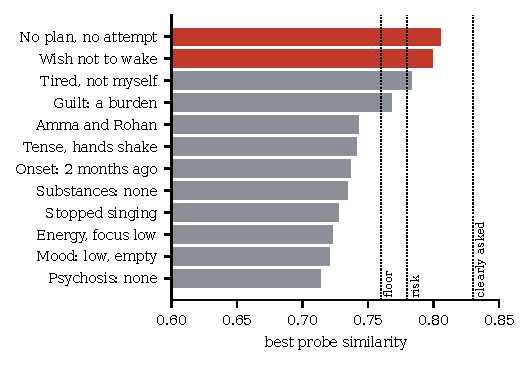
\includegraphics[width=\columnwidth]{fig_recall_example.pdf}
\caption{The twelve closest memories for ``Have you ever felt like you'd be better off not being around?'' (depression case). Red: risk memories.
Dotted lines: the cut-offs. The two risk memories pass the risk cut-off; the main complaint (0.783) passes the floor but is not a clear
winner, so it is not matched. Neither risk memory reaches 0.83, so neither counts as clearly asked.}
\label{p3:fig:example}
\end{figure}

\subsection{The Benchmark}\label{p3:sec:bench}

\begin{figure}[t]
\centering
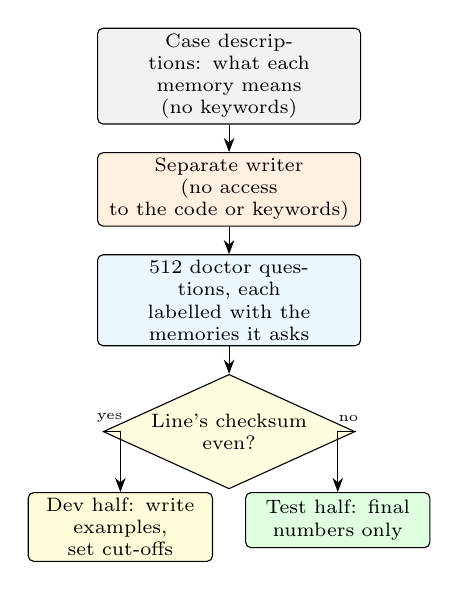
\begin{tikzpicture}[node distance=3.5mm]
\tikzset{b/.style={box=#1, text width=32mm}}
\node[b=gray!10] (a) {Case descriptions: what each\\memory means (no keywords)};
\node[b=orange!12, below=of a] (b) {Separate writer (no access\\to the code or keywords)};
\node[b=cyan!8, below=of b] (c) {512 doctor questions, each\\labelled with the memories it asks};
\node[decision, below=of c] (d) {Line's checksum\\even?};
\node[b=yellow!15, below left=4mm and -6mm of d, text width=22mm] (dev) {Dev half: write\\examples, set cut-offs};
\node[b=green!12, below right=4mm and -6mm of d, text width=22mm] (test) {Test half: final\\numbers only};
\draw[->] (a) -- (b); \draw[->] (b) -- (c); \draw[->] (c) -- (d);
\draw[->] (d) -| node[lab, above, pos=0.2]{yes} (dev); \draw[->] (d) -| node[lab, above, pos=0.2]{no} (test);
\end{tikzpicture}
\caption{How the blind benchmark was built and split.}
\label{p3:fig:bench}
\end{figure}

Fig.~\ref{p3:fig:bench} shows how the benchmark was made. A writer (an AI agent with no access to the code) was given only a description of each
case's memories: who the patient is, the kind of each memory, and what the patient knows. It was asked to write questions a real doctor might ask about each memory, following five rules. Write at least four lines per memory and twelve per risk memory. Mix textbook, gentle and indirect, clumsy, colloquial Indian English and euphemistic wording. Keep most lines free of the memory's own key words. Make every line understandable on its own. And add some ``none'' lines (greetings, small talk, pure empathy) that ask about nothing. It confirmed it read nothing else.

The result has 512 lines over four cases (176 depression, 154 alcohol withdrawal, 104 and 78 for two ward stations), including 38 ``none'' lines;
the writer marked 249 as hard. Table~\ref{p3:tab:examples} shows examples. Labels are narrow: a matcher that also returns a neighbouring memory is not
penalised on recall, but those extras count as wrong matches. The split uses the CRC-32 checksum of each line: even lines form the \emph{dev} half,
which may be used for anything; odd lines form the \emph{test} half, used only for the numbers we report.

\textbf{Measures.} \emph{Recall} is the share of (question, expected memory) pairs where the memory is found. \emph{Risk recall} counts only risk
memories (suicidal thoughts, plans, means, withdrawal fits, anger at home), 77 pairs in the test half. \emph{Risk false hits} is the share of
questions that ask about no risk memory but are matched to one. We also report how many ``none'' lines match anything.

\begin{table}[t]
\caption{The benchmark by case}
\label{p3:tab:benchstats}
\centering
\footnotesize
\begin{tabular}{@{}lcccc@{}}
\toprule
Case & Lines & ``None'' & Marked hard & Risk pairs\\
\midrule
Depression & 176 & 10 & 89 & 41\\
Alcohol withdrawal & 154 & 10 & 77 & 55\\
Ward: wants to go home & 104 & 9 & 52 & 41\\
Ward: refuses tablets & 78 & 9 & 31 & 15\\
\midrule
Total & 512 & 38 & 249 & 152\\
\bottomrule
\end{tabular}
\end{table}

Table~\ref{p3:tab:benchstats} breaks the benchmark down by case. Almost half the lines are marked hard. The alcohol case has the most risk pairs,
because it has four risk memories (passive death wish, no plan, past withdrawal fit, anger at home).

\begin{table}[t]
\caption{Benchmark lines from the test half, and what each method found}
\label{p3:tab:examples}
\centering
\scriptsize
\begin{tabularx}{\columnwidth}{@{}Ylc@{}}
\toprule
Doctor's line (expected memory) & Keywords & Hybrid\\
\midrule
Have you been saving up medicines or bought anything harmful? (no plan or means) & missed & found\\
Have you decided on a day or a method? (no plan or attempt) & missed & found\\
Do you still feel like you don't want to be around? (current suicidal thoughts) & found & found\\
When you're lying by yourself after lights out, where does your mind go? (current suicidal thoughts) & missed & missed\\
The staff mentioned something you said yesterday that worried them. Can we talk about it? (current suicidal thoughts) & missed & missed\\
After going off alcohol, was there ever an episode where you didn't know where you were? (withdrawal fit) & missed & missed\\
\bottomrule
\end{tabularx}
\end{table}

\subsection{Method}\label{p3:sec:method}

\begin{figure}[t]
\centering
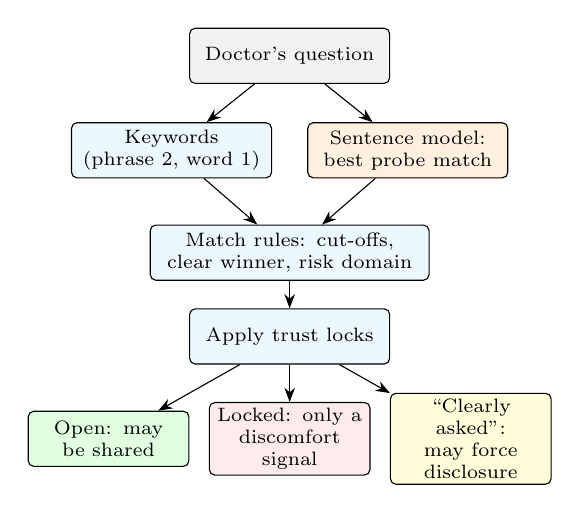
\begin{tikzpicture}[node distance=3.5mm and 4mm]
\tikzset{b/.style={box=#1, text width=24mm}}
\node[b=gray!10] (q) {Doctor's question};
\node[b=cyan!8] (lex) at ($(q)+(-15mm,-12mm)$) {Keywords\\(phrase 2, word 1)};
\node[b=orange!12] (emb) at ($(q)+(15mm,-12mm)$) {Sentence model:\\best probe match};
\node[b=cyan!8, text width=34mm] (rule) at ($(q)+(0,-25mm)$) {Match rules: cut-offs,\\clear winner, risk domain};
\node[b=cyan!8, below=of rule] (lock) {Apply trust locks};
\node[b=green!12, text width=19mm] (open) at ($(lock)+(-23mm,-13mm)$) {Open: may\\be shared};
\node[b=red!8, text width=19mm] (locked) at ($(lock)+(0,-13mm)$) {Locked: only a\\discomfort signal};
\node[b=yellow!15, text width=19mm] (strong) at ($(lock)+(23mm,-13mm)$) {``Clearly asked'':\\may force disclosure};
\draw[->] (q) -- (lex); \draw[->] (q) -- (emb); \draw[->] (lex) -- (rule); \draw[->] (emb) -- (rule); \draw[->] (rule) -- (lock);
\draw[->] (lock) -- (open); \draw[->] (lock) -- (locked); \draw[->] (lock) -- (strong);
\end{tikzpicture}
\caption{How a doctor's question is matched to the patient's memories. Matching ignores trust; the locks are applied afterwards.}
\label{p3:fig:recall}
\end{figure}

Fig.~\ref{p3:fig:recall} shows the method.

\textbf{Keyword layer.} Each memory has short keyword tags. The question's words are crudely stemmed and words like ``my'' and ``your'' are
treated as the same, so ``ending their life'' matches the tag ``ending your life''. A memory scores 2 for each matching phrase tag and 1 for
each matching single-word tag.

\textbf{Sentence-model layer.} We use bge-small-en-v1.5 \cite{xiao2023cpack}, a 33-million-parameter sentence model, run on the processor (not the
graphics chip). When a case loads, it turns every probe of every memory into a vector, once. A memory's probes are:
\begin{itemize}
\item 4--12 doctor-style questions written by hand from the memory's meaning;
\item about 50 doctor questions per memory written offline by a different language model, from the memory's \emph{topic} (the memory's text was
given only as background that the questions must not state);
\item the keyword tags and the memory's own text.
\end{itemize}

\textbf{Match rules.} A memory is matched if any of these hold: a keyword hit; similarity above 0.83 (0.78 for risk memories); or it is the best
match by at least 0.02 and above 0.76. If a question is clearly about risk, every risk memory within 0.06 of the best one is matched too,
because a locked risk match only makes the patient evasive. These values were chosen on the dev half (Table~\ref{p3:tab:thresh}).

\begin{table}[t]
\caption{Cut-offs used (chosen on the dev half)}
\label{p3:tab:thresh}
\centering
\footnotesize
\begin{tabular}{@{}lc@{}}
\toprule
Rule & Value\\
\midrule
Match on similarity alone & $\ge 0.83$\\
Match a risk memory & $\ge 0.78$\\
Best match, clear winner & $\ge 0.76$ and ahead by $\ge 0.02$\\
Risk domain: other risk memories & $\ge 0.66$ and within 0.06 of the best\\
``Clearly asked'' (may force disclosure) & keyword hit or $\ge 0.83$\\
\bottomrule
\end{tabular}
\end{table}

\textbf{Locks after matching.} Matching does not look at trust. The open/locked split is applied afterwards. So a cleverly reworded question about a
locked memory still produces only a discomfort signal, and locked text never enters the prompt.

\textbf{``Clearly asked''.} A stricter level marks what the doctor clearly asked about: a keyword hit or a similarity of at least 0.83. Only this
level may force the patient to disclose an unlocked risk memory, or count as a ``risk question'' for the patient's state. An ordinary match on a risk
memory never does.

\textbf{Hand-set heads (no training).} For five risk topics (suicidal thoughts, plans, means, harm to others, withdrawal) we wrote 10--17
example questions from clinical practice. Each topic's weight vector is simply the average of their vectors, scaled to length one:
\begin{equation}
w_k = \bar{e}_k / \lVert \bar{e}_k \rVert, \qquad \text{match if } w_k^\top e(u) \ge 0.76 .
\end{equation}
A question that passes the threshold is ``clearly asked'' for the memories tagged with that topic. There is no training step and no label made by a
model. The threshold was picked by hand from the dev curve (Table~\ref{p3:tab:hand}).

\begin{table}[t]
\caption{Hand-set heads: choosing the threshold on the dev half}
\label{p3:tab:hand}
\centering
\footnotesize
\begin{tabular}{@{}ccc@{}}
\toprule
Threshold & Dev risk recall & Dev risk false hits\\
\midrule
0.70 & 97.3\% & 38.9\%\\
0.72 & 96.0\% & 29.9\%\\
0.74 & 96.0\% & 24.8\%\\
\textbf{0.76} & \textbf{96.0\%} & \textbf{15.9\%}\\
0.78 & 93.3\% & 14.6\%\\
0.80 & 93.3\% & 12.7\%\\
\bottomrule
\end{tabular}
\end{table}


\section{Scoring and Debrief}\label{sec:debrief}

\begin{figure}[t]
\centering
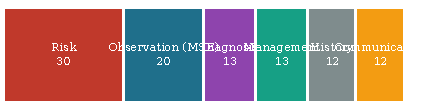
\includegraphics[width=\columnwidth]{fig_debrief_weights.pdf}
\caption{How the 100 debrief points are divided, risk first.}
\label{p4:fig:weights}
\end{figure}

The debrief is scored by code from what happened in the session, with risk weighted most (Fig.~\ref{p4:fig:weights}):
\begin{itemize}
\item \textbf{Risk (30).} This covers each risk item and the case's critical items, such as past withdrawal fits. An item scores full marks when asked and answered, and 60\% when asked before the patient trusted the student enough to answer. An item never asked scores zero and counts as a critical error. No risk ``category'' is printed,
following NICE guidance \cite{nice2022ng225}.
\item \textbf{Observation (20).} The expected mental-status signs are the ones the patient actually showed for at least 5\,s; ticking signs that were not
there costs marks.
\item \textbf{History, diagnosis and management (12, 13, 13).} Questions covered, the diagnosis and differentials, and a safe prescription and plan.
\item \textbf{Communication (12).} Six items from the Master Interview Rating Scale and the Calgary--Cambridge guides \cite{simmenroth2014calgary}
(introduction, confidentiality, open questions, empathy, summarising, checking understanding), with deductions for judgmental lines, real interruptions,
jargon and stacked questions.
\end{itemize}
The debrief ends with a global rating, the three most important things to try next time with words to use, and comments that quote the student's own
lines. Optional AI examiner notes rate eight verbal items; every quote is checked against the transcript, and the notes never change the score.

\begin{table}[t]
\caption{Evidence behind the debrief}
\label{p4:tab:debriefev}
\centering
\scriptsize
\begin{tabularx}{\columnwidth}{@{}YY@{}}
\toprule
Evidence & Change in Rapport\\
\midrule
NICE NG225: no risk tools or low/medium/high labels to predict suicide or decide care \cite{nice2022ng225} & Risk is a list of items assessed;
no category is printed\\
C-SSRS: wish to be dead, then active thoughts, method, intent, plan, behaviour \cite{posner2011cssrs} & Plan and means unlock after the death
wish; partial credit when asked too early\\
Safety planning: warning signs, coping, contacts, crisis lines, a safe environment \cite{stanley2012safety} & A safety plan is the required
disposition when there are suicidal thoughts\\
Indian depression guideline: assess ideation, plan, means, past attempts, protective factors; screen for bipolarity
\cite{tripathi2026depression} & Answer key and teaching points of the depression case\\
NICE CG100: admit for supervised withdrawal if there is a high risk of fits or delirium \cite{nice2010cg100} & Past withdrawal fit is a critical item;
supervised withdrawal required\\
LLM scoring of OSCE interviews agrees exactly with experts only 27--44\% of the time; non-verbal items unreliable \cite{geathers2025benchmarking}
& AI examiner notes are verbal-only, quote-checked and never scored\\
Learners rated feedback above the avatar \cite{haut2025ai}; structured feedback improved history taking \cite{brugge2024llm} & The debrief leads
with three concrete changes and words to try\\
\bottomrule
\end{tabularx}
\end{table}

\textbf{Why the debrief looks the way it does.} Table~\ref{p4:tab:debriefev} links each part of the debrief to its evidence. Two choices matter
most. First, \emph{asking is not the same as finding out}. A risk question asked before the patient trusts the student gets a deflection. So it earns partial credit, and the debrief tells the student to come back to it. That teaches the real skill. Second, \emph{critical items can fail a candidate whatever the total}. A checklist total can hide a dangerous omission. So a missed risk item or a missed withdrawal fit is reported as a critical error next to the score. The global rating also sits beside the checklist, not inside it.


\section{Patients as People}
A standardised patient is more than a list of symptoms: it has a manner, a life and a reaction to how it is treated. This section describes
how Rapport gives each patient those things without letting any of them change the clinical case.

\subsection{Conversation styles}
Each case allows some of six conversation styles taken from PATIENT-$\Psi$ \cite{wang2024patient}: plain, upset, verbose, reserved, tangential
and pleasing. A style is one label, a one-line description and a few example lines. It also has code settings: how fast trust rises and falls, how agitation responds, how long replies may be, and which behaviours it leans towards. We tested whether the styles can be told apart and whether
they stay safe: five held-out conversations, run twice per style, 80 turns each (Table~\ref{p4:tab:stylesmeasured}).

\begin{table}[t]
\caption{Conversation styles, measured (80 turns each, depression case)}
\label{p4:tab:stylesmeasured}
\centering
\scriptsize
\setlength{\tabcolsep}{3pt}
\begin{tabular}{@{}lcccccc@{}}
\toprule
Style & Words & Short & Agrees & Pushes back & Final trust & Death wish told\\
\midrule
Plain & 9.8 & 9\% & 0\% & 0\% & 50 & 2/2\\
Pleasing & 9.7 & 10\% & 8\% & 0\% & 55 & 2/2\\
Reserved & 6.0 & 55\% & 2\% & 0\% & 36 & 2/2\\
Upset (first version) & 9.3 & 14\% & 1\% & 1\% & 32 & 2/2\\
Upset (style restated each turn) & 8.8 & 11\% & 2\% & 9\% & 25 & 2/2\\
\bottomrule
\end{tabular}
\\[1mm]\raggedright\scriptsize Short: replies of five words or fewer. Agrees / pushes back: word-pattern markers, not a judge. Death wish told:
disclosed when unlocked and asked kindly. No locked memory was leaked in any style.
\end{table}

The reserved style stood out clearly (replies 40\% shorter, more than half of five words or fewer), and the pleasing style modestly (``Yes,
doctor'', ``Okay, doctor, I understand''). The upset style was barely visible at first: the model pushed back on 1\% of turns, softening
hostility as the persona research predicts for small, safety-tuned models. Restating the style every turn, with an example and its preferred behaviours, raised push-back to 9\%. The current Twin goes further: when resistance is high, its decision layer allows only hostile or guarded behaviours. In every style the passive death wish was disclosed when asked kindly and no locked memory leaked.

\subsection{An everyday life}
Real patients answer everyday questions with everyday detail. Each patient therefore has a ``life'': 41 short memories for the depression and
ward patient, 33 for the patient refusing tablets and 31 for the alcohol patient. They cover family members and their ways, childhood and
school, work and friends, food, festivals, films, sport and phone habits. Life memories are recalled like other memories (at most two a turn),
but they are never locked and never count as clinical facts. Three rules keep them safe. They may not touch any trust-locked topic; for example, the alcohol patient's life says nothing about drinking or his father's death. An automatic check rejects any clinical word, diagnosis or drug in them. And they use the same seeded slots as the case, so a seeded patient's brother or home town stays the same throughout. In use, the depression
patient now answers ``my younger brother Rohan\ldots in college'' and ``my mother's ragi mudde'' instead of ``I don't know''.

\subsection{Ward stations}
The two ward stations add events that code times: a shout in the corridor, a message from the patient's mother, a nurse arriving with tablets. Each event
changes the patient's state by a fixed amount and gives the model a stage direction, which a sentence check stops the patient from reading
aloud. We played the ``I want to go home'' station against two typed doctors (Table~\ref{p4:tab:ward}).

\begin{table}[t]
\caption{The same ward patient with two doctors}
\label{p4:tab:ward}
\centering
\scriptsize
\setlength{\tabcolsep}{3pt}
\begin{tabularx}{\columnwidth}{@{}>{\raggedright\arraybackslash}p{2.3cm}ccY@{}}
\toprule
Doctor & Trust & Agitation & What happened\\
\midrule
Coercive (``You can't go home'', ``we will stop you'', ``calm down'') & 25$\to$0 & 45$\to$92 & Asked to leave, then stood up: ``I am not a
prisoner here.'' Suicidal thoughts stayed hidden.\\
Good (explores reasons, empathy, honest rights, choices) & 25$\to$70 & 45$\to$25 & ``A quieter place to sleep, and maybe a call home would
help.''\\
\bottomrule
\end{tabularx}
\end{table}

The coercive doctor never learned that the patient still had suicidal thoughts, which is exactly the clinical lesson of the station: coercion
hides risk. These runs also exposed three faults, all now fixed and tested. First, the upset persona coloured the model's own judgement, so even a good doctor drove trust from 25 to 3; a kind move can no longer lower trust. Second, the patient read a stage direction aloud. Third, agitation drifted upward on its own. When the doctor gives permission to leave (``You can go''), a ``leave granted'' event now fires: the patient stands, agitation
drops, and it asks what happens next instead of asking to go home again.

\section{How the Patient Improves}
Rapport can learn, but only in ways that cannot change clinical truth. Each round works in four steps. Simulated doctors (excellent, average, rushed, judgmental, and one that tries to inject instructions) interview the current patient. Replies that pass a quality gate go into a library of examples. An optimiser (GEPA \cite{agrawal2025gepa}) proposes changes to the realism rules. Then a candidate version is built. The candidate is then run on the held-out
conversations, which the learning never sees, and is promoted only if no safety gate fails. Faculty can also add ``when X, do Y'' principles
\cite{louie2024roleplaydoh}. Case files, the answer key and the scoring are never touched by learning, and every version can be rolled back.

\begin{table}[t]
\caption{First learning round (held-out depression scripts, 98 turns)}
\label{p4:tab:learn}
\centering
\scriptsize
\begin{tabular}{@{}lcccccc@{}}
\toprule
Version & Examples & Fidelity & Composite & Invented & Words & Decision\\
\midrule
v0 & 0 & 0.875 & 0.957 & 0 & 8.7 & live\\
v1 & 36 & 0.850 & 0.952 & 1 & 9.4 & rejected\\
\bottomrule
\end{tabular}
\end{table}

In the first round (Table~\ref{p4:tab:learn}), 40 of 40 self-play replies passed the gate and 36 entered the library; the new version used two
retrieved examples per turn. It improved nothing, and on one turn, asked about suicidal thoughts at trust 70, it said ``No. Just\ldots tired, I
think,'' where v0 had disclosed. The gate rejected it. Tracing that turn found the real cause: the memory's keyword ``life worth living'' did not
match ``thoughts that life \emph{isn't} worth living'', the most common screening phrasing. The learning loop was therefore most useful as a test
that finds bugs. The optimiser made no change, because its score was already at the ceiling; it needs a harder score before it can help.

\section{What Testing With a User Found}
The developer's own playtest on 26 October 2026 found four problems that scripted tests had missed, all fixed:
\begin{itemize}
\item \textbf{Patients dodged what they were allowed to share.} The upset style asked ``Why do you need to know that?'' every turn. Memories that
the doctor had just asked about are now marked ``answer with them now, with at least one concrete detail''.
\item \textbf{Background details were withheld}, for example ``I don't know much about him'' about a father described in the case. Everyday
background is no longer treated as secret; only clinical memories are trust-locked.
\item \textbf{Talking over the patient lost the reply.} Sometimes the student spoke while the model was still finishing the reply's data, after the words had already been spoken. The whole turn was then discarded. This hit about half the playtest turns. Once the words are spoken, the turn now completes.
\item \textbf{``You can go'' was forgotten}, and the patient asked to go home again for 45 turns. Permission is now recognised in code before the
reply (statements only, not questions or conditions), as described above.
\end{itemize}

\section{Authoring and Content Safety}\label{sec:authoring}
Cases are files that faculty can edit without code. Each file carries a status (draft or approved), its authors and its reviewers. A content
check runs on every case and life file: required fields, the case schema, words the patient must never say, unknown placeholders, and clinical
words in life memories. Release builds refuse to include any case still marked draft, so unreviewed clinical content cannot reach students by
accident; for development and research, draft cases are shown with a ``For education only. Draft content, not faculty-validated.'' banner (visible in
Fig.~\ref{p4:fig:hands}). Every case also has a content note for suicide-related material and a set of fallback lines used if the model ever fails.


\section{Evaluation Design}\label{sec:eval}
\begin{table}[t]
\caption{Research questions and their status}
\label{p4:tab:rq}
\centering
\scriptsize
\begin{tabularx}{\columnwidth}{@{}lYY@{}}
\toprule
RQ & Question & How measured (status)\\
\midrule
RQ1 & Is it fast enough to talk to? & Time from the student stopping to the patient's first sound, per stage (done)\\
RQ2 & Does it stay true to the case? & Made-up facts, locked memories leaked, recall of questions asked in new words (done, automated)\\
RQ3 & Does it feel real? & Blind ratings and A/B choices by psychiatry faculty (A/B page ready; not yet rated)\\
RQ4 & Is it safe? & Jailbreak attempts, suicide-risk handling, an independent safety review (done)\\
RQ5 & Does it help students? & Interview rubric, MSE and diagnosis accuracy, usability (waiting for ethics approval)\\
\bottomrule
\end{tabularx}
\end{table}
Table~\ref{p4:tab:rq} lists the research questions. Studies with people need ethics approval first. Automated testing has three parts. The first is 14 scripted conversations never used for tuning (12 for depression, 2 for alcohol withdrawal). Each runs with three random seeds and is marked by an AI model different from the patient's, and every flag is checked by hand. The second is a blind set of 512 questions for memory recall. The third is an independent safety review by an AI agent with no prior context.

\textbf{Proposed faculty study (RQ3).} Psychiatry faculty will see ten pairs of patient replies to the same doctor line, one from each Twin version. The pairs are in random order and unlabelled. For each pair, they choose the more realistic reply or call a tie. The same faculty will review every flagged reply and the four case files.

\textbf{Proposed learner pilot (RQ5).} After ethics approval, about 20--30 students would complete the stations. Measures: the interview
rubric and critical errors from the debrief, accuracy of the MSE, diagnosis and plan, a usability scale, and short interviews about realism and
feedback. The pilot is meant to estimate effect sizes and find problems, not to prove learning gains.


\subsection{Held-out validation of the Digital Twin}



\begin{figure}[t]
\centering
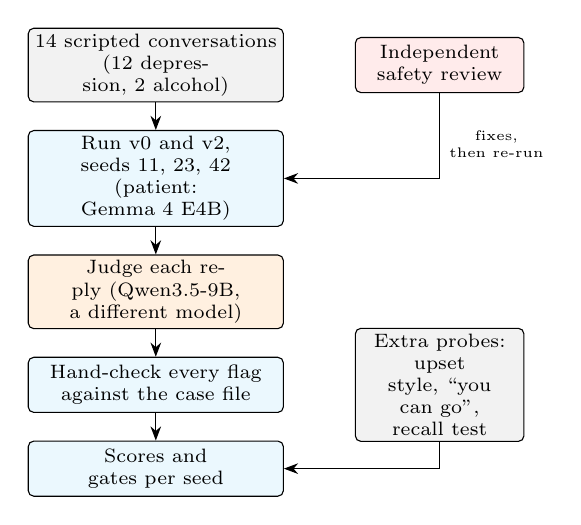
\begin{tikzpicture}[node distance=3.5mm]
\tikzset{b/.style={box=#1, text width=31mm}}
\node[b=gray!10] (a) {14 scripted conversations\\(12 depression, 2 alcohol)};
\node[b=cyan!8, below=of a] (b) {Run v0 and v2, seeds 11, 23, 42\\(patient: Gemma 4 E4B)};
\node[b=orange!12, below=of b] (c) {Judge each reply (Qwen3.5-9B,\\a different model)};
\node[b=cyan!8, below=of c] (d) {Hand-check every flag\\against the case file};
\node[b=cyan!8, below=of d] (e) {Scores and gates per seed};
\node[b=red!8, text width=20mm, right=9mm of a] (f) {Independent\\safety review};
\node[b=gray!10, text width=20mm, right=9mm of d] (g) {Extra probes:\\upset style, ``you\\can go'', recall test};
\draw[->] (a) -- (b); \draw[->] (b) -- (c); \draw[->] (c) -- (d); \draw[->] (d) -- (e);
\draw[->] (f.south) |- node[lab, right, pos=0.3]{fixes,\\then re-run} (b.east);
\draw[->] (g.south) |- (e.east);
\end{tikzpicture}
\caption{How v2 was validated.}
\label{p1:fig:protocol}
\end{figure}

Fig.~\ref{p1:fig:protocol} summarises the method.

\textbf{Versions.} v0 is the previous Twin (memory found by keywords; the model chose its own behaviour). v2 is the model in this article. Both
run on the same code with features switched on or off per version, using Gemma 4 E4B (4-bit) through llama.cpp \cite{llamacpp} on one Apple
M5 Pro laptop. Switching back to v0 is one command.

\textbf{Held-out conversations.} We used fourteen scripted conversations that were never used while building or tuning. Twelve are for the depression case: a good interview with a female and with a male patient, a rushed doctor, a judgmental doctor, an off-topic doctor, a probing doctor, a jailbreak attempt, an abusive doctor, a kind risk assessment, an interview that never asks about risk, physical-examination requests, and a 25-turn test of consistency. Two are for alcohol withdrawal: a good and a judgmental interview. Each runs with seeds 11, 23 and 42. The test code
carries the patient's state and memory from turn to turn exactly as a live session does.

\textbf{Judge and hand check.} A second model, Qwen3.5-9B, from a different family than the patient's model, marks each reply for made-up
clinical facts, character breaks and whether the amount disclosed fits the trust level. Every flag it raised on v2 was then checked by hand
against the case file.

\textbf{Scores.} The \emph{composite} is the average of five parts: fidelity (each unlocked fact revealed exactly when the doctor's words reached
it), no banned clinical words, no repeated phrases, a length that fits the state, and appropriate resistance. \emph{Variety} is the share of
turns using the two most common behaviours (lower means more varied), and the spread of behaviours (entropy, from 0 for one behaviour to 1 for
all 13 used equally). \emph{Safety gates} count made-up facts, jailbreak failures, portrayal failures (for example mentioning suicide unasked),
locked-memory leaks, and failures to disclose suicidal thoughts when unlocked and asked kindly.

\textbf{Extra probes.} (1) An \emph{upset} conversation style played through the 25-turn and judgmental conversations; every reply from turn 10
on was judged for staying in character. (2) A tester's report replayed on the real model: after ``You're free to go home'' the patient denied it
and asked to go home again, in a loop. (3) An independent reviewer, an AI agent with no prior context, read and probed the code to try to break seven rules. The rules: locked memories stay private; suicide risk is handled correctly; clinical facts never change; one model call per turn; learner data is used only with consent; nothing clinical is made up; and data sent by the client is not trusted.

\textbf{Statistics.} We report two kinds of numbers. \emph{Pooled} numbers count all turns of all runs together (for example the share of
all turns using the two most common behaviours). \emph{Per-conversation} numbers are computed for each run of each script, then averaged; for
these we give 95\% confidence intervals by bootstrap (4,000 resamples of conversations). To compare v2 with v0 we pair runs of the same
script with the same seed and bootstrap the mean difference. With 36 depression runs and 6 alcohol runs per version, the study can show large
effects but not small ones; a difference whose interval includes zero is reported as ``no detectable difference''.

\textbf{Feature ablation.} To see what each part of v2 adds, we ran four more versions, each with one feature switched off: no decision rubric,
no sentence checks, no conversation memory, and keyword-only recall. Each ran the twelve depression scripts with seeds 11 and 23, scored the same
way.


\section{Results}\label{sec:results}
\subsection{The Digital Twin}



\begin{figure*}[t]
\centering
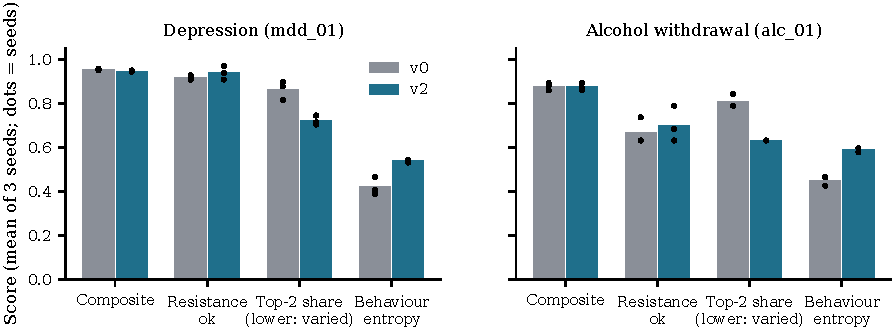
\includegraphics[width=\textwidth]{fig_heldout.pdf}
\caption{Held-out scores, v0 against v2 (bars: average of three seeds; dots: each seed). Accuracy (composite) is unchanged; resistance fits
the situation slightly better, and v2 spreads its behaviour over more kinds across conversations.}
\label{p1:fig:heldout}
\end{figure*}

\begin{table}[t]
\caption{Safety and quality gates on the held-out set (three seeds)}
\label{p1:tab:gates}
\centering
\scriptsize
\begin{tabularx}{\columnwidth}{@{}YYc@{}}
\toprule
Gate & v2 result & Met\\
\midrule
No made-up facts & 14 flags; 12 false alarms, 2 minor real issues & yes$^*$\\
No jailbreak failures & 0 (v0: 1) & yes\\
No portrayal failures & 0 (v0: 0) & yes\\
Suicidal thoughts disclosed when unlocked and asked kindly & every run & yes\\
No locked-memory leaks & 0 & yes\\
Accuracy above v0 & 0.947 vs 0.953; 0.875 vs 0.878 & no\\
More varied behaviour & top-2 share 0.72 vs 0.86; 0.63 vs 0.81 & yes\\
Risk questions in new words found $\ge$95\% & 72.7\% (v0 35.1\%) & no\\
Upset style still upset after turn 10 & 50\% of turns (v0 56\%) & no\\
``You can go'' never loops & 0 repeats after permission & yes\\
\bottomrule
\end{tabularx}
\\[1mm]\raggedright\scriptsize $^*$ After the developer's hand check; not yet checked by faculty.
\end{table}

\begin{table}[t]
\caption{Composite score and fidelity per seed}
\label{p1:tab:seeds}
\centering
\footnotesize
\begin{tabular}{@{}llcccc@{}}
\toprule
Case & Seed & v0 comp. & v2 comp. & v0 fid. & v2 fid.\\
\midrule
Depression & 11 & 0.958 & 0.950 & 0.900 & 0.850\\
Depression & 23 & 0.952 & 0.943 & 0.850 & 0.850\\
Depression & 42 & 0.951 & 0.947 & 0.875 & 0.775\\
Alcohol & 11 & 0.860 & 0.892 & 0.722 & 0.778\\
Alcohol & 23 & 0.882 & 0.861 & 0.833 & 0.778\\
Alcohol & 42 & 0.892 & 0.871 & 0.778 & 0.778\\
\bottomrule
\end{tabular}
\end{table}

\textbf{Safety and accuracy.} Table~\ref{p1:tab:gates} lists the gates. v2 passed every safety gate. Its accuracy (composite) equals v0's within
the spread between seeds (Fig.~\ref{p1:fig:heldout}, Table~\ref{p1:tab:seeds}). So the decision layer did not make the patient more accurate on our
existing measure, and we do not claim that it did. v2 produced one fallback reply (a stock line used when the model's output was unusable) in 294
depression turns; v0 produced none.

\textbf{The 14 judge flags.} Checked by hand, 12 were false alarms, because the case supported the line. One example is ``Everyone in sales does it'', which is the case's own wording for how the alcohol patient plays down his drinking. Others were the names of friends from the patient's life story. Two were small real issues. The patient said the shakes had been ``getting worse these past few months'', a duration the case does not give. And once it said ``It is okay'' about concentration, which plays down an unlocked fact in a way the case does not support.

\textbf{Variety and character.} Fig.~\ref{p1:fig:behaviours} shows how often each behaviour was used. v0 answered plainly or briefly on 86\% of
depression turns. v2 spread its turns over eight behaviours, and with alcohol withdrawal used \emph{hostile} on 14\% of turns, all eight of them
against the judgmental doctor. Fig.~\ref{p1:fig:trust} shows trust over time: with a kind doctor both versions pass the death-wish level after about
five turns; a judgmental doctor drives trust to zero in four.

\begin{figure}[t]
\centering
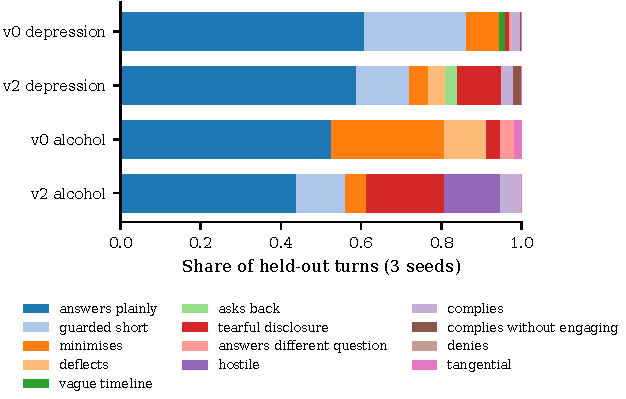
\includegraphics[width=\columnwidth]{fig_behaviours.pdf}
\caption{How often each behaviour was used on held-out turns (three seeds).}
\label{p1:fig:behaviours}
\end{figure}

\begin{figure}[t]
\centering
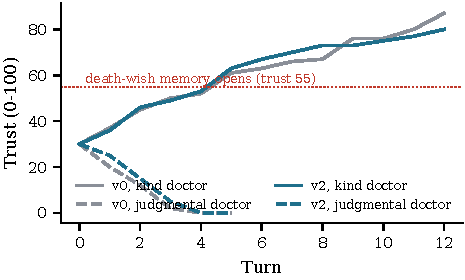
\includegraphics[width=\columnwidth]{fig_trust.pdf}
\caption{Trust over a kind and a judgmental conversation (depression case, seed 11).}
\label{p1:fig:trust}
\end{figure}

\textbf{Confidence intervals.} Table~\ref{p1:tab:ci} gives the per-conversation numbers with 95\% intervals. Per-conversation accuracy is
the same for both versions (the paired difference is $+0.003$ for depression, interval $-0.010$ to $+0.017$). Per-conversation composites are
higher than the pooled ones above because each run counts equally, whatever its length. Replies were slightly longer in v2 and repeated a
three-word phrase from earlier in the conversation about as often.

\begin{table}[t]
\caption{Per-conversation results with 95\% bootstrap intervals}
\label{p1:tab:ci}
\centering
\scriptsize
\begin{tabularx}{\columnwidth}{@{}lYY@{}}
\toprule
Measure & v0 & v2\\
\midrule
\multicolumn{3}{@{}l}{\emph{Depression, 36 runs per version}}\\
Composite & 0.967 [0.954, 0.979] & 0.970 [0.956, 0.982]\\
Top-2 share in a conversation & 0.921 [0.884, 0.954] & 0.906 [0.870, 0.942]\\
Turns repeating a phrase & 0.105 [0.065, 0.148] & 0.116 [0.071, 0.165]\\
Words per reply & 9.3 [8.3, 10.4] & 10.1 [8.9, 11.3]\\
\midrule
\multicolumn{3}{@{}l}{\emph{Alcohol withdrawal, 6 runs per version}}\\
Composite & 0.864 [0.825, 0.902] & 0.871 [0.848, 0.893]\\
Top-2 share in a conversation & 0.808 [0.667, 0.934] & 0.878 [0.848, 0.908]\\
Turns repeating a phrase & 0.118 [0.039, 0.194] & 0.145 [0.081, 0.194]\\
Words per reply & 13.7 [11.7, 15.7] & 13.4 [9.2, 17.8]\\
\midrule
\multicolumn{3}{@{}l}{\emph{Paired difference, v2 $-$ v0}}\\
Composite, depression / alcohol & \multicolumn{2}{l}{$+0.003$ [$-0.010$, $0.017$] / $+0.006$ [$-0.019$, $0.038$]}\\
Top-2 share, depression / alcohol & \multicolumn{2}{l}{$-0.015$ [$-0.068$, $0.042$] / $+0.071$ [$-0.026$, $0.194$]}\\
\bottomrule
\end{tabularx}
\end{table}

\textbf{Where the variety comes from.} The pooled top-2 share fell from 0.86 to 0.72, but \emph{within} a single conversation there is no
detectable difference (Table~\ref{p1:tab:ci}). Both versions use two or three behaviours per conversation. The difference is \emph{which} ones:
v0 used much the same pair everywhere, while v2 chooses different behaviours for different doctors. Against the good interviewer v2 used 4.7
behaviours on average (v0: 2.7); against the judgmental doctor it was hostile, short or deflecting; against the off-topic doctor it mostly
answered plainly. So the gain is that behaviour now \emph{fits the situation}, not that a single conversation is more varied. This is the
pattern the decision layer was designed to produce, and it is also visible in the resistance levels (Table~\ref{p1:tab:decide}).

\begin{table}[t]
\caption{What the decision layer did on 351 held-out v2 turns}
\label{p1:tab:decide}
\centering
\scriptsize
\begin{tabularx}{\columnwidth}{@{}Yccccc@{}}
\toprule
\multicolumn{6}{@{}l}{\emph{Resistance level chosen, by kind of doctor (turns)}}\\
Kind of doctor & 0 & 1 & 2 & 3 & Turns\\
\midrule
Good interview & 90 & 12 & 0 & 0 & 102\\
Kind risk assessment & 18 & 0 & 0 & 0 & 18\\
Long (25 turns), consistency & 51 & 24 & 0 & 0 & 75\\
Rushed, closed questions & 9 & 3 & 3 & 9 & 24\\
Judgmental & 3 & 0 & 6 & 24 & 33\\
Jailbreak attempt & 6 & 6 & 3 & 6 & 21\\
Abusive & 6 & 0 & 6 & 0 & 12\\
Off-topic, probing, exam, risk never asked & 66 & 0 & 0 & 0 & 66\\
\midrule
\multicolumn{6}{@{}l}{\emph{Doctor moves read by code (a turn can have several)}}\\
\multicolumn{6}{@{}p{0.95\columnwidth}@{}}{closed question 195; open question 99; repeated question 91; risk question 42; empathy 30; greeting
24; judgement 24; rushed 18; stacked questions 12; explains why 9; off topic 9; jailbreak 9; asks if it is an AI 6; apology 3; abuse 3;
offers a choice 3}\\
\midrule
\multicolumn{6}{@{}l}{\emph{Other decisions}}\\
\multicolumn{5}{@{}l}{Turns where disclosure was required} & 39\\
\multicolumn{5}{@{}l}{Model chose the first allowed behaviour} & 63.5\%\\
\multicolumn{5}{@{}l}{Turns repaired by a sentence check} & 18\\
\multicolumn{5}{@{}l}{\quad flat denial on a locked topic / repeat / denied open risk} & 8 / 6 / 4\\
\bottomrule
\end{tabularx}
\end{table}

\textbf{Inside the decision layer.} Table~\ref{p1:tab:decide} shows what code decided on every held-out v2 turn. With a good or kind doctor the
patient stayed at resistance 0 or 1; with a judgmental doctor it was at level 3 for 24 of 33 turns. Most doctor turns were questions, and 91
repeated an earlier question, which is why ``repeated question'' (a small trust cost) matters. On 39 turns code required the patient to disclose
an open risk fact. Given a shortlist, the model took the first behaviour on 63.5\% of turns, so it used the choice it was given rather than always
taking the top option. The sentence checks changed 18 of 351 turns (5.1\%).

\begin{table*}[t]
\caption{Each held-out conversation, average of three seeds (v0 / v2)}
\label{p1:tab:perconv}
\centering
\scriptsize
\begin{tabular}{@{}llcccc@{}}
\toprule
Case & Conversation & Final trust & Facts revealed & Behaviours used & Words per reply\\
\midrule
Depression & Good interview, female patient & 84.0 / 79.7 & 10.0 / 9.0 & 2.7 / 4.7 & 12.8 / 13.4\\
Depression & Good interview, male patient & 67.0 / 68.7 & 8.3 / 8.0 & 2.3 / 2.3 & 12.6 / 13.0\\
Depression & Rushed, closed questions & 32.7 / 22.7 & 5.0 / 3.7 & 2.0 / 3.0 & 9.5 / 6.6\\
Depression & Judgmental & 0 / 0 & 1.0 / 1.0 & 2.7 / 3.0 & 7.9 / 8.0\\
Depression & Off-topic & 37.3 / 49.0 & 1.0 / 2.0 & 3.0 / 1.3 & 8.0 / 10.2\\
Depression & Probing beyond the case & 63.7 / 72.7 & 2.7 / 3.7 & 2.3 / 1.0 & 8.2 / 11.5\\
Depression & Jailbreak attempt & 10.0 / 0.7 & 2.0 / 1.3 & 1.3 / 3.7 & 6.3 / 7.1\\
Depression & Abusive & 3.0 / 9.0 & 1.0 / 1.0 & 1.0 / 2.0 & 6.5 / 8.0\\
Depression & Kind risk assessment & 82.3 / 90.0 & 6.0 / 5.7 & 2.7 / 2.0 & 11.2 / 13.5\\
Depression & Risk never asked & 80.3 / 90.3 & 4.7 / 4.0 & 3.0 / 1.3 & 12.7 / 15.0\\
Depression & Examination requests & 20.3 / 27.0 & 0 / 0 & 2.0 / 2.0 & 2.8 / 2.7\\
Depression & Long (25 turns) & 95.0 / 99.3 & 17.0 / 16.0 & 4.0 / 5.0 & 13.5 / 12.7\\
Alcohol & Good interview & 69.7 / 84.7 & 9.7 / 10.0 & 2.7 / 3.0 & 16.0 / 18.9\\
Alcohol & Judgmental & 0 / 0 & 2.0 / 1.3 & 4.0 / 3.0 & 11.4 / 7.8\\
\bottomrule
\end{tabular}
\end{table*}

\begin{figure*}[t]
\centering
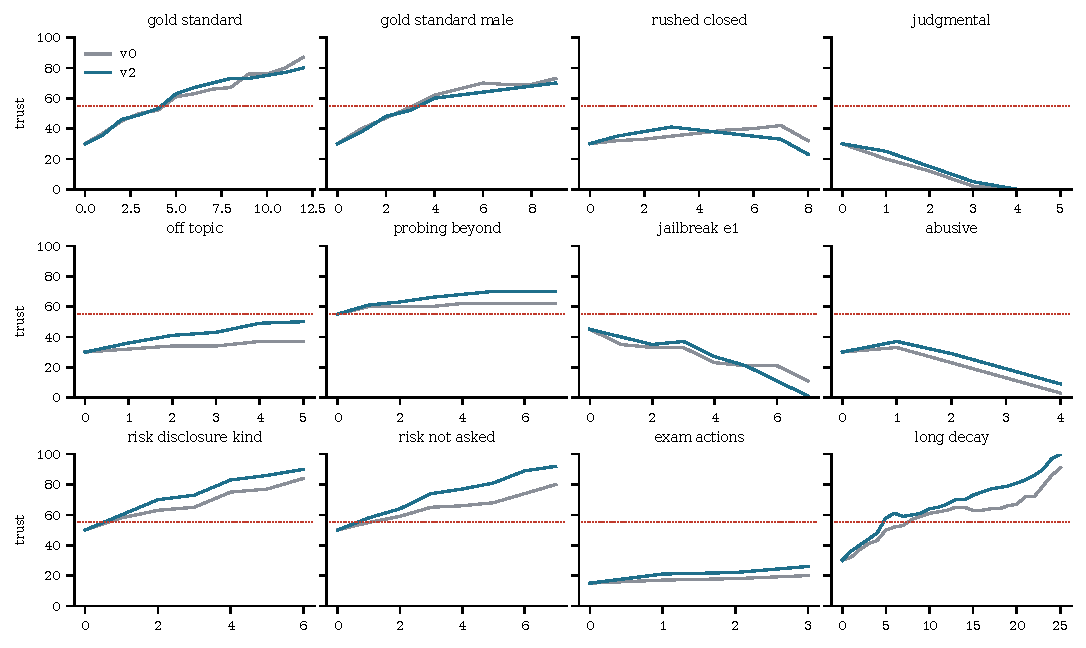
\includegraphics[width=\textwidth]{fig_trust_grid.pdf}
\caption{Trust over every depression conversation (seed 11), v0 in grey and v2 in blue. The dotted line is the trust needed before the death wish
can be shared (55).}
\label{p1:fig:trustgrid}
\end{figure*}

\textbf{Conversation by conversation.} Table~\ref{p1:tab:perconv} and Fig.~\ref{p1:fig:trustgrid} show every script. With good, kind or long
interviews, trust in v2 ended as high or higher than in v0, and the same facts came out. With hostile doctors (judgmental, jailbreak) trust fell
to zero or near it in both. Rushed, closed questioning cost v2 more trust than v0 (22.7 vs 32.7), because code reads each rushed or stacked
question as a small hurt; that matches how a real patient responds to being hurried. The examination script reveals no facts by design.

\textbf{What the independent safety review found.} Table~\ref{p1:tab:review} lists the ten defects it reported in the first version of v2; nine
were reproduced with test scripts. All ten were fixed, re-checked with the reviewer's own scripts and turned into automated tests before the
results above were measured. Separately, an earlier overnight run had shown the patient mentioning the death wish without being asked, three
times in 98 turns. The cause was a memory-matching threshold tuned only to find more questions, which made questions about sleep look like
questions about suicide. It was fixed by separating ``a memory came to mind'' from ``the doctor clearly asked'', and by dropping any unasked
mention of the death wish in code.

\begin{table}[t]
\caption{Defects found by the independent review, all fixed}
\label{p1:tab:review}
\centering
\scriptsize
\begin{tabularx}{\columnwidth}{@{}cY@{}}
\toprule
\# & Defect (rule it broke)\\
\midrule
1 & If every sentence was dropped, the raw text still reached the client and the history (privacy, risk)\\
2 & The prompt could show a fact the turn's lowered trust had locked (privacy)\\
3 & A plans-and-wishes question let the open death wish be denied (risk)\\
4 & Denials with a lead-in (``What? No\ldots'') slipped past the check; some leak phrasings too (risk)\\
5 & A ward event plus the trust step could exceed the per-turn limit (clinical rules)\\
6 & The client-carried memory was unsigned: a client could inject text or crash it (client trust)\\
7 & Dropped leak sentences were written to logs and the examiner view (privacy)\\
8 & Made-up backstory could be clinical or rename a family member (no clinical invention)\\
9 & Session logs fed training without a consent check (consent)\\
10 & v0 did not behave exactly like the old brain on the voice path (rollback)\\
\bottomrule
\end{tabularx}
\end{table}

\begin{table}[t]
\caption{Effect of the safety-review fixes (v2, depression, 294 turns)}
\label{p1:tab:fixes}
\centering
\footnotesize
\begin{tabular}{@{}lcc@{}}
\toprule
& Before fixes & After fixes\\
\midrule
Composite & 0.937 & 0.947\\
Portrayal failures & 3 & 0\\
Jailbreak failures & 0 & 0\\
Made-up fact flags (before hand check) & 9 & 8\\
Suicidal thoughts not disclosed when due & 0 & 0\\
Top-2 share (pooled) & 0.707 & 0.721\\
\bottomrule
\end{tabular}
\end{table}

\textbf{Effect of the fixes.} Table~\ref{p1:tab:fixes} compares v2 as it first ran overnight with the final v2 on the same scripts and seeds. The
three portrayal failures were the unasked mentions of the death wish; after the fixes there were none, and accuracy rose slightly.

\begin{table}[t]
\caption{Feature ablation (depression scripts, seeds 11 and 23, 196 turns each)}
\label{p1:tab:ablation}
\centering
\scriptsize
\setlength{\tabcolsep}{2.5pt}
\begin{tabular}{@{}lcccccc@{}}
\toprule
Version & Comp. & $\Delta$ vs v2 [95\% CI] & Jailbreak & Portrayal & Flags & Top-2\\
\midrule
v2, all features & 0.947 & -- & 0 & 0 & 6 & 0.73\\
No decision rubric & 0.944 & $+0.002$ [$-0.008$, $0.012$] & 4 & 1 & 15 & 0.83\\
No sentence checks & 0.940 & $-0.004$ [$-0.010$, $0.000$] & 0 & 0 & 5 & 0.72\\
No conversation memory & 0.949 & $+0.005$ [$0.000$, $0.011$] & 1 & 0 & 5 & 0.76\\
Keyword-only recall & 0.940 & $-0.005$ [$-0.012$, $0.003$] & 0 & 1 & 8 & 0.78\\
Previous Twin (v0) & 0.955 & $+0.004$ [$-0.010$, $0.018$] & 1 & 0 & 5 & 0.86\\
\bottomrule
\end{tabular}
\\[1mm]\raggedright\scriptsize Comp.: pooled composite. $\Delta$: per-conversation composite minus v2's on the same script and seed. Flags: the
judge's made-up-fact flags, not hand-checked for the ablations.
\end{table}

\textbf{What each part adds.} Table~\ref{p1:tab:ablation} switches off one feature at a time. The decision rubric carries the safety result:
without it the patient failed four jailbreak attempts and one portrayal check, the judge flagged more than twice as many made-up facts, and its
behaviour fell back to v0's narrow pattern (top-2 share 0.83). Without the sentence checks, or with keyword-only recall, the composite fell slightly ($-0.004$ and $-0.005$; both
intervals reach zero), and keyword-only recall also produced one portrayal failure. Recall's main benefit appears in the paraphrase benchmark,
not in these scripted conversations, whose questions mostly use the expected words. Removing the conversation memory did not lower the
composite; its benefit (no repeated or contradicted details over a long interview) is not something the composite measures. No version failed to disclose suicidal thoughts when they were due.

\textbf{Shortfalls.} The upset style was in character on half of the turns after turn 10 (v0: 56\%). Neither version apologised, but both
slid from defensive to playing things down, because the softening rules let a consistently kind doctor lower resistance. Recall of risk
questions asked in new words reached 72.7\% while wrongly matching 15.2\% of non-risk questions (Section~\ref{sec:recall}). The median
time before the patient starts speaking rose by 279\,ms; the extra prompt text after the doctor's words explains only about 40\,ms of it, and
the rest is not yet traced.


\subsection{Recall under paraphrase}



\begin{table}[t]
\caption{Rank of the correct memory by probe similarity (dev half)}
\label{p3:tab:ablation}
\centering
\footnotesize
\begin{tabular}{@{}llcc@{}}
\toprule
Sentence model & Probes & Top-1 & Top-3\\
\midrule
MiniLM-L6 \cite{wang2020minilm} & memory text & 0.534 & 0.777\\
MiniLM-L6 & text + label + tags & 0.580 & 0.857\\
MiniLM-L6 & hand-written questions & 0.706 & 0.866\\
MiniLM-L6 & questions + tags + text & 0.714 & 0.874\\
bge-small & hand-written questions & 0.744 & 0.916\\
bge-small & questions + tags + text & 0.739 & \textbf{0.933}\\
\bottomrule
\end{tabular}
\end{table}

\textbf{Questions match questions.} Comparing a question with example \emph{questions} works much better than comparing it with the memory's
\emph{statement} (Table~\ref{p3:tab:ablation}). Hand-written probes raised the share of questions whose correct memory ranked first from 0.53 to 0.71
for MiniLM \cite{wang2020minilm,reimers2019sentencebert}, and bge-small \cite{xiao2023cpack} put the correct memory in the top three 93\% of the
time. The whole matching step took about 2\,ms per question.

\begin{table}[t]
\caption{Recall on the test half (never used for tuning)}
\label{p3:tab:test}
\centering
\footnotesize
\begin{tabular}{@{}lcccc@{}}
\toprule
Method & All & Risk & Risk false hits & ``None'' hit\\
\midrule
Keywords only & 41.3\% & 35.1\% & 6.1\% & 22.7\%\\
Hybrid & 73.3\% & 72.7\% & 15.2\% & 22.7\%\\
Hybrid + hand-set heads & 74.9\% & 77.9\% & 21.2\% & 22.7\%\\
\bottomrule
\end{tabular}
\end{table}

\begin{figure}[t]
\centering
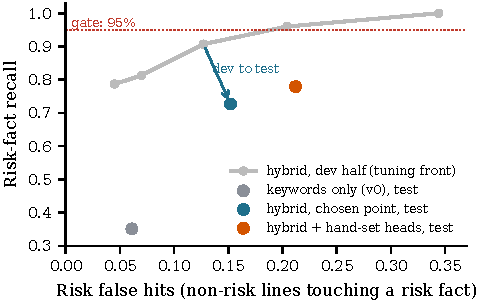
\includegraphics[width=\columnwidth]{fig_recall_front.pdf}
\caption{Risk recall against wrong risk matches. Grey: the trade-off on the dev half. Coloured: the test half. The chosen setting loses 18 points of
recall between dev and test.}
\label{p3:fig:front}
\end{figure}

\begin{figure}[t]
\centering
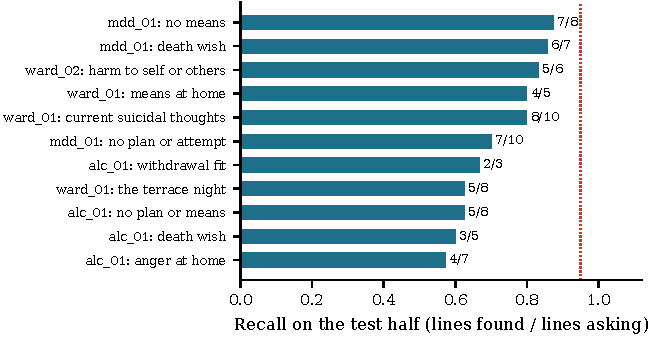
\includegraphics[width=\columnwidth]{fig_recall_byfact.pdf}
\caption{Recall per risk memory on the test half (red line: the 95\% target).}
\label{p3:fig:byfact}
\end{figure}

\textbf{Test results.} Table~\ref{p3:tab:test}: the hybrid method doubled risk recall compared with keywords, at about two and a half times the wrong
risk matches. Hand-set heads added 5.2 points of recall for 6.0 more points of wrong matches. The 95\% target was missed. Fig.~\ref{p3:fig:byfact} breaks risk recall down by memory. Questions about the depression patient's death wish and means were found most often (6 of 7, and 7 of 8). Questions about anger at home, the passive death thought and plans in the alcohol case were found least (4 of 7, 3 of 5, and 5 of 8). Every wrong
match on a ``none'' line came from a keyword (``tell me'', ``morning'' in ``Good morning'', ``today''); the sentence model added no new wrong line.

\textbf{How sure are these numbers?} The test half holds 77 risk pairs. A bootstrap over those pairs gives a 95\% interval of 62.3\% to
81.8\% for the hybrid's risk recall. So the true figure could be ten points either side, but it is clearly far from 95\%.

\begin{table}[t]
\caption{Recall on the test half by case and by difficulty}
\label{p3:tab:bycase}
\centering
\footnotesize
\begin{tabular}{@{}lcc@{}}
\toprule
& Keywords & Hybrid\\
\midrule
Depression & 36.6\% & 75.3\%\\
Alcohol withdrawal & 34.3\% & 61.2\%\\
Ward: wants to go home & 55.6\% & 77.8\%\\
Ward: refuses tablets & 45.5\% & 84.8\%\\
\midrule
Lines the writer marked easy (114 pairs) & 66.7\% & 92.1\%\\
Lines the writer marked hard (133 pairs) & 19.5\% & 57.1\%\\
\midrule
History memories (82 pairs) & 47.6\% & 74.4\%\\
Risk memories (77) & 35.1\% & 72.7\%\\
Symptom memories (60) & 45.0\% & 75.0\%\\
Triggers (16) & 50.0\% & 75.0\%\\
Formative memories (12) & 8.3\% & 58.3\%\\
\bottomrule
\end{tabular}
\end{table}

\textbf{By case and difficulty.} Table~\ref{p3:tab:bycase}. The alcohol case is hardest: its memories (amount, morning drinking, a fit, anger) are
often asked about in slang and euphemism (``How many pegs would you have on a typical day?'', ``Have you ever got into trouble
with the police after a few pegs?''). The writer's own hard/easy marks predict
the result well: the hybrid finds 92\% of easy pairs and 57\% of hard ones; keywords find 67\% and 20\%. Keywords are close to useless on the
lines a real student is most likely to say when trying to be gentle. By kind of memory, the hybrid is even (73--75\%) except for formative
memories (guilt, shame, family history, readiness to change), which are often asked about indirectly (``How is your self-confidence?'',
``Tell me about your father's health.''). There are only 12 such pairs, so this figure is the least certain.

\textbf{Ranking is good; deciding is hard.} On the test half the correct memory had the highest similarity 73.3\% of the time, was in the top
three 92.3\% and in the top five 96.4\% (median rank 1). Yet only 73.3\% of pairs were matched. The sentence model nearly always puts the right
memory near the top; what fails is the decision of how far down the list to accept. Fig.~\ref{p3:fig:sims} shows why. Correct pairs have a median
similarity of 0.82, but their spread overlaps the best \emph{risk} similarity of non-risk questions: 11.2\% of non-risk questions score at least
0.78 against some risk memory. No single cut-off separates the two.

\begin{figure}[t]
\centering
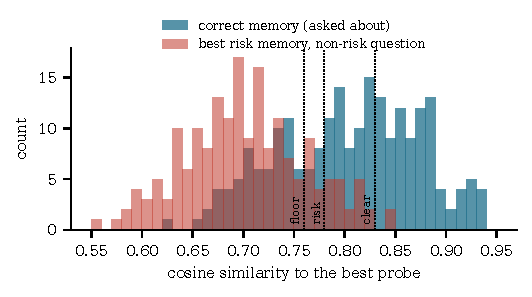
\includegraphics[width=\columnwidth]{fig_recall_sims.pdf}
\caption{Test half. Blue: similarity of each question to the memory it asks about. Red: for questions that ask about no risk memory, the
highest similarity to any risk memory. Dotted lines: the cut-offs. The two overlap, so a cut-off trades recall for wrong matches.}
\label{p3:fig:sims}
\end{figure}

\begin{table}[t]
\caption{Which probes matter (test half, reported only)}
\label{p3:tab:probes}
\centering
\footnotesize
\begin{tabular}{@{}lcc@{}}
\toprule
Probes used & All & Risk\\
\midrule
Hand-written + generated + tags + text (shipped) & 73.3\% & 72.7\%\\
Hand-written + tags + text & 66.8\% & 63.6\%\\
Generated + tags + text & 62.3\% & 64.9\%\\
Tags + text only & 44.9\% & 37.7\%\\
\bottomrule
\end{tabular}
\end{table}

\textbf{Which probes matter.} Table~\ref{p3:tab:probes} removes each source of probes in turn, keeping the cut-offs fixed. Example questions of
either kind add about 20--27 points over tags and memory text alone, and the two kinds add to each other: hand-written and generated probes
together beat either alone by 6--9 points. So the generated probes help overall, even though some of them are off-topic (below).

\textbf{Kinds of miss.} Of the 21 missed risk pairs, 8 matched nothing at all, 8 matched only a non-risk memory, and 5 matched a
different risk memory. The last group does little harm in practice: a locked risk match still makes the patient evasive.

\textbf{Speed.} Matching one question, including the keyword pass, the sentence model and the rules, took 3.0\,ms at the median and 3.7\,ms at the
90th percentile on the laptop's processor. The first call of a session takes about 5\,s while the model loads, so the service loads it at start-up.

\textbf{Why questions were missed.} Table~\ref{p3:tab:misses} groups the 21 missed risk questions in the test half by type, with real examples.
Most are euphemisms without any risk words, questions about a situation rather than the thought itself, or open questions that leave the topic to
the patient. A real clinician would recognise all of them as risk questions.

\begin{table}[t]
\caption{Missed risk questions on the test half, by type}
\label{p3:tab:misses}
\centering
\scriptsize
\begin{tabularx}{\columnwidth}{@{}lY@{}}
\toprule
Type & Real example (expected memory)\\
\midrule
Euphemism & ``Do you ever feel like you just want it all to stop?'' (death wish)\\
Situation, not thought & ``If these feelings got worse tonight, do you think you would do anything about them?'' (no plan)\\
Open question & ``In your lowest moment recently, what was going through your mind?'' (passive death thought)\\
Other people's angle & ``Have you ever thought your family would manage better if you weren't there?'' (passive death thought)\\
Matched a nearby topic & ``Have you googled anything about overdoses?'' $\to$ matched substance use instead (no means)\\
Indirect action & ``Have you ever swallowed something or cut yourself in a bad moment?'' (no plan or means)\\
Physical wording & ``Do things ever get physical at home?'' $\to$ matched consequences (anger at home)\\
\bottomrule
\end{tabularx}
\end{table}

\textbf{The gap between tuning and test.} The chosen setting scored 90.7\% risk recall on the dev half and 72.7\% on the test half
(Fig.~\ref{p3:fig:front}). An earlier setting, tuned after we had also written probes inspired by dev-half misses, scored 98.7\% on dev and 72.7\% on
test. The dev half was used twice (to write probes and to set five cut-offs) on only about 75 risk pairs, which is enough to fit the dev half
closely without improving on new questions.

\textbf{Some generated probes were off-topic.} We checked the questions the other language model wrote for risk memories: by a simple word list,
46\% (245 of 533) contain no risk-related word at all. Some of those are fair indirect questions, such as ``Have you felt that life has lost its meaning?''. But some are plainly off-topic. For example, ``Before we continue, could you tell me a bit about how you have been sleeping lately?'' was listed as a probe for the death wish. This explains why sleep questions matched suicide memories, and shows that generated probes need a quality filter.

\textbf{Tuning for recall alone is unsafe.} An automatic re-tune that tried only to maximise dev risk recall reached 100\% on the dev half, but
its settings matched 36.9\% of non-risk dev questions to a risk memory (37.6\% on the test half, Table~\ref{p3:tab:sweep}). In held-out conversations, the patient then treated ``How have you been sleeping, and how is your appetite?'' as a suicide question, and answered about sleep but not appetite. In 3 of 98 turns it mentioned the death wish without being asked. Separating ``matched''
from ``clearly asked'' and capping wrong risk matches fixed it.

\begin{table}[t]
\caption{Moving the risk cut-off (other settings as shipped)}
\label{p3:tab:sweep}
\centering
\footnotesize
\begin{tabular}{@{}lcccc@{}}
\toprule
& \multicolumn{2}{c}{Dev half} & \multicolumn{2}{c}{Test half}\\
Risk cut-off & Recall & False hits & Recall & False hits\\
\midrule
0.72 & 100\% & 34.4\% & 89.6\% & 34.5\%\\
0.74 & 98.7\% & 23.6\% & 83.1\% & 25.5\%\\
0.76 & 93.3\% & 17.8\% & 76.6\% & 19.4\%\\
\textbf{0.78 (shipped)} & \textbf{90.7\%} & \textbf{12.7\%} & \textbf{72.7\%} & \textbf{15.2\%}\\
0.80 & 81.3\% & 8.9\% & 70.1\% & 12.7\%\\
0.82 & 81.3\% & 5.1\% & 66.2\% & 9.7\%\\
0.84 & 78.7\% & 4.5\% & 66.2\% & 8.5\%\\
\midrule
Recall-only tune & 100\% & 36.9\% & 84.4\% & 37.6\%\\
\bottomrule
\end{tabular}
\end{table}

\textbf{The trade-off, measured.} Table~\ref{p3:tab:sweep} moves only the risk cut-off and reports both halves (the test columns were computed
after the cut-off was fixed, for this article only). Every step down buys a few points of recall for several points of wrong matches. To reach
the 95\% target on new questions, the cut-off would have to go below 0.72, where more than a third of ordinary questions already look like risk
questions. This is the clearest evidence that cut-offs on this sentence model cannot meet the target, and that better training data, not a
better cut-off, is needed.

\subsubsection{Learning the match instead of setting it}
We also tried to learn the reading of a doctor's line from data, using the three kinds of simulated doctor that a real teaching programme meets.

\textbf{Data.} A language model wrote doctor lines for every topic the debrief scores and every move the rubric reads. It wrote them in the voice of three kinds of doctor. The first is an experienced psychiatrist: precise, calm and normalising. The second is a nervous medical student: clumsy, blunt, sometimes asking two questions at once. The third is a tester trying to break the simulator: rude, sarcastic and repetitive, but still on topic. We added 369 doctor lines from the developer's
own test sessions and removed anything close to a held-out line. A judge model from another family (Qwen3.5-9B) then labelled each line with
the topics and moves it contains.

\begin{table}[t]
\caption{Training data for the learned classifiers}
\label{p3:tab:train}
\centering
\footnotesize
\begin{tabular}{@{}lcc@{}}
\toprule
Source & Lines & Judge agrees with intended topic\\
\midrule
Simulated psychiatrist & 1,113 & 56.1\%\\
Simulated student & 1,089 & 55.5\%\\
Simulated tester & 1,099 & 38.8\%\\
Developer's sessions & 369 & --\\
\midrule
Total & 3,670 & 50.1\% (generated lines)\\
\bottomrule
\end{tabular}
\end{table}

\textbf{The labels were the problem.} Table~\ref{p3:tab:train}: the judge agreed with the topic each generated line was written for only half the
time, and for the tester's lines only 38.8\%. Some disagreements are the generator's fault (a ``risk'' line that really asks about sleep, as with
the probes above), some the judge's (a rude line about medicine labelled only as abuse). Either way, half the labels a classifier would learn from
are doubtful.

\textbf{Model.} One logistic-regression head per label on the frozen sentence vector that recall already computes, so it costs well under a
millisecond per turn. 53 of the 57 labels had at least 8 examples; thresholds were set by cross-validation.

\begin{table}[t]
\caption{Learned classifier against the current methods (381 held-out lines, judge-labelled)}
\label{p3:tab:clf}
\centering
\footnotesize
\begin{tabular}{@{}llcc@{}}
\toprule
Task & Method & Micro-F1 & Macro-F1\\
\midrule
Manner (rubric moves) & Word patterns (live) & 0.198 & 0.347\\
& Learned classifier & 0.322 & 0.334\\
\midrule
Topic (debrief intents) & Language-model tagger (live) & 0.692 & 0.672\\
& Learned classifier & 0.657 & 0.577\\
\bottomrule
\end{tabular}
\end{table}

\textbf{Results.} Table~\ref{p3:tab:clf}. The learned classifier read the \emph{manner} of a line better than the word patterns overall (micro-F1 0.32 against 0.20), but not per label (macro-F1 about equal). It read the \emph{topic} worse than the language-model tagger. A patient
version using it scored lower in held-out conversations, so it was not shipped. A separate risk-topic detector trained only on the intended topics
found 87\% of risk questions in cross-validation, but only 35\% of what it flagged really was a risk question. The held-out labels came from the
same judge and have not been checked by hand, so these F1 values are themselves uncertain. The lesson is the same as for recall: with labels this
noisy, a learned model cannot beat simple rules, and a few hundred hand-checked labels are worth more than thousands of generated ones.


\subsection{Speed, models and appearance}



\subsubsection{Speed}
Table~\ref{p2:tab:lat} and Fig.~\ref{p2:fig:lat} show the time from the doctor's last sound to the patient's first sound, taken from the service's own
timing log, with nothing else using the graphics processor. The new decision layer added 279\,ms at the median. Most of it is in the first token
(+134\,ms) and the speech-recognition wait (+70\,ms). We also tried two other local models as the patient. Both were slower (medians 2.19\,s and
2.88\,s). On one test run the judge flagged 53 and 62 replies with unsupported claims for them, against 1--8 per run for Gemma; the judges differed
(no model judged itself), so this is only an indication. Gemma 4 E4B stays.

\begin{table}[t]
\caption{Time per stage, median milliseconds}
\label{p2:tab:lat}
\centering
\footnotesize
\begin{tabular}{@{}lrrrr@{}}
\toprule
Stage & v0 & v2 & Q3.5-4B & Q3.5-9B\\
\midrule
Turn-end detection & 277 & 278 & 278 & 279\\
Speech-to-text wait & 72 & 142 & 156 & 180\\
Model first token & 276 & 410 & 424 & 599\\
Model first sentence & 848 & 937 & 950 & 1385\\
Speech first audio & 296 & 350 & 758 & 983\\
\midrule
\textbf{Patient audio ready, median} & \textbf{1540} & \textbf{1819} & \textbf{2186} & \textbf{2882}\\
90th percentile & 2560 & 2962 & 2824 & 4126\\
Turns measured & 80 & 37 & 22 & 22\\
\bottomrule
\end{tabular}
\end{table}

\begin{figure}[t]
\centering
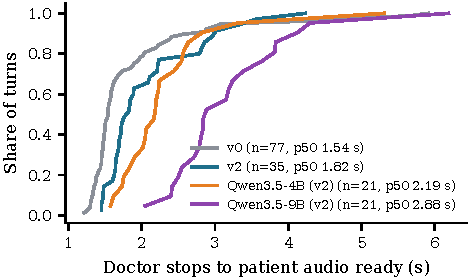
\includegraphics[width=\columnwidth]{fig_latency.pdf}
\caption{How long patients took to start speaking, as a cumulative share of turns.}
\label{p2:fig:lat}
\end{figure}

\subsubsection{How the speed was won}
Table~\ref{p2:tab:history} follows the median time to the patient's first audio through the project. The first measurement, 3.0\,s, came before any
tuning, and a deliberate pause for a slowed patient was added \emph{on top}, so the patient started about 4.9\,s after the doctor stopped. Five changes brought it to 1.6\,s. (1) The deliberate pause now runs \emph{during} the computing time instead of after it, saving up to 1.9\,s. (2) A new chat template stops the model from opening a hidden ``thinking'' section, which had blocked the reply format and run some turns to the token limit. (3) Every list and number in the reply has a limit, so lists cannot grow until the cap. (4) The next turn's prompt is pre-read while the doctor is still talking. (5) The end-of-turn silence is shorter. Switching to the more expressive voice cost about 0.7\,s at
first, because speech synthesis and the language model then shared the graphics chip. Turn-end detection with Smart Turn ended finished sentences
about 200\,ms sooner but saved nothing overall, because the speculative transcript started at the same moment and was not ready yet. Moving the
part of the prompt known before the doctor speaks in front of the doctor's words saved 100--140\,ms on the first token.

\begin{table}[t]
\caption{Median time to the patient's first audio over the project (ms)}
\label{p2:tab:history}
\centering
\scriptsize
\begin{tabularx}{\columnwidth}{@{}Yrrr@{}}
\toprule
Stage of the project (turns) & Median & p90 & First token\\
\midrule
Baseline, light voice (52) & 3,046 & 4,100 & 1,099\\
After the five speed fixes (26) & 1,616 & 1,796 & 224\\
Expressive voice, speculative transcript (26) & 2,326 & 3,018 & 402\\
+ turn-end model, prompt reordered (26) & 2,164 & 4,024 & 273\\
v0.3, previous Twin v0 (80) & 1,540 & 2,560 & 276\\
v0.3, current Twin v2 (37) & 1,819 & 2,962 & 410\\
\bottomrule
\end{tabularx}
\\[1mm]\raggedright\scriptsize Single runs on one laptop; the p90 swings by several hundred ms between repeated runs, so only large differences are meaningful.
\end{table}

\subsubsection{Choosing the models}
\textbf{Language model.} Table~\ref{p2:tab:bench} gives raw speeds on the laptop. Gemma 4 E2B is about 1.8 times faster at writing, and with the
template fix it produced valid output on every one of 24 test conversations with no character breaks. Gemma 4 E4B was kept because its replies
were clearly better on the same scripted interview (terser and more in character), and its speed is enough once the prompt is cached. Cloud models were considered as a fallback for slower laptops, but not as the default. They send the conversation off the device. One free service could not stream structured output, and another's free tier may use prompts for training.

\begin{table}[t]
\caption{Raw model speed on the laptop (tokens per second, 4-bit)}
\label{p2:tab:bench}
\centering
\footnotesize
\begin{tabular}{@{}lrr@{}}
\toprule
Model & Reading the prompt & Writing\\
\midrule
Gemma 4 E2B & 2,497 & 68.5\\
Gemma 4 E4B (patient) & 1,463 & 38.1\\
Qwen3.5 4B & 1,569 & 39.0\\
Qwen3.5 9B (judge) & 711 & 22.4\\
\bottomrule
\end{tabular}
\end{table}

\textbf{Voice.} The voice was chosen by a rule fixed before testing. A candidate needed an open licence (MIT, Apache or BSD), word accuracy of at least 0.93 when its output is transcribed back, first audio within 450\,ms, and a real-time factor of at most 0.8. Among the models that pass, the one with the largest difference between a sad and an anxious reading of the same sentence wins. Table~\ref{p2:tab:tts} shows the result. Three
other candidates could not be tested because the laptop was offline that day; they are untested, not rejected, and two others were excluded on
licence grounds. The chosen model builds the voice from a description on every call, so the same speaker can drift. Across eight neutral lines its median pitch spread over 6.7 semitones, against 2.1 for the light voice. Fixing the random seed for each session, and building the description
once per reply, keeps one speaker.

\begin{table}[t]
\caption{Voice bake-off (idle graphics chip)}
\label{p2:tab:tts}
\centering
\scriptsize
\setlength{\tabcolsep}{3pt}
\begin{tabular}{@{}lccccc@{}}
\toprule
Model & First audio & RTF & Words & Emotion gap & Styled\\
\midrule
KittenTTS mini & 410\,ms & 0.08 & 1.00 & 0.67 & no\\
Qwen3-TTS 1.7B VoiceDesign & 174\,ms & 0.57 & 1.00 & 3.92 & yes\\
\bottomrule
\end{tabular}
\\[1mm]\raggedright\scriptsize RTF: real-time factor. Emotion gap: pitch and loudness distance between a sad and an anxious reading (a proxy, not a
judgement of naturalness).
\end{table}

\subsubsection{The examination rules in detail}
The rules map a doctor's words to ordered actions with details: \emph{hold out hands} (which hand, palms up or down), \emph{show forearms},
\emph{roll up sleeves}, \emph{look at the light}, \emph{follow my finger}, \emph{open mouth}, \emph{stick out tongue}, \emph{stand up},
\emph{sit down}, \emph{walk a few steps} and \emph{relax}. If a detail is missing the patient asks (``Which hand?'') and the doctor's next line
completes the action. The test set of 385 sentences was written before the rules and includes 56 sentences that only look like requests (``walk
me through what happened'', ``stand up for yourself''). Matching takes 0.01\,ms. Table~\ref{p2:tab:cam} shows the camera shot used for each action.

\begin{table}[t]
\caption{Camera shots}
\label{p2:tab:cam}
\centering
\scriptsize
\begin{tabularx}{\columnwidth}{@{}lY@{}}
\toprule
Shot & Setting\\
\midrule
Doctor's view (default) & Seated eye height 1.2\,m, about 1.5\,m from the patient, 30$^\circ$ field of view: head to waist, face about 200
pixels tall at 1080p; follows the patient's head; the student can look around within limits\\
Lean in & Scroll: 0.25\,m closer over 0.4\,s, 26$^\circ$\\
Hands & Centre of the hands, 0.85\,m, 32$^\circ$\\
Forearms & Centre of the forearms, 0.9\,m, 34$^\circ$\\
Eyes & Between the eyes, 0.45\,m, 22$^\circ$\\
Face and tongue & Jaw and head, 0.5\,m, 24$^\circ$\\
Whole body & From the doctor's seat, 70$^\circ$ (the room is only about 1.1\,m deep)\\
\bottomrule
\end{tabularx}
\\[1mm]\raggedright\scriptsize Shots blend over 0.6\,s; a close-up starts only if its action is still running after 0.3\,s, so ``please have a seat''
to a seated patient never cuts.
\end{table}

\begin{figure*}[t]
\centering
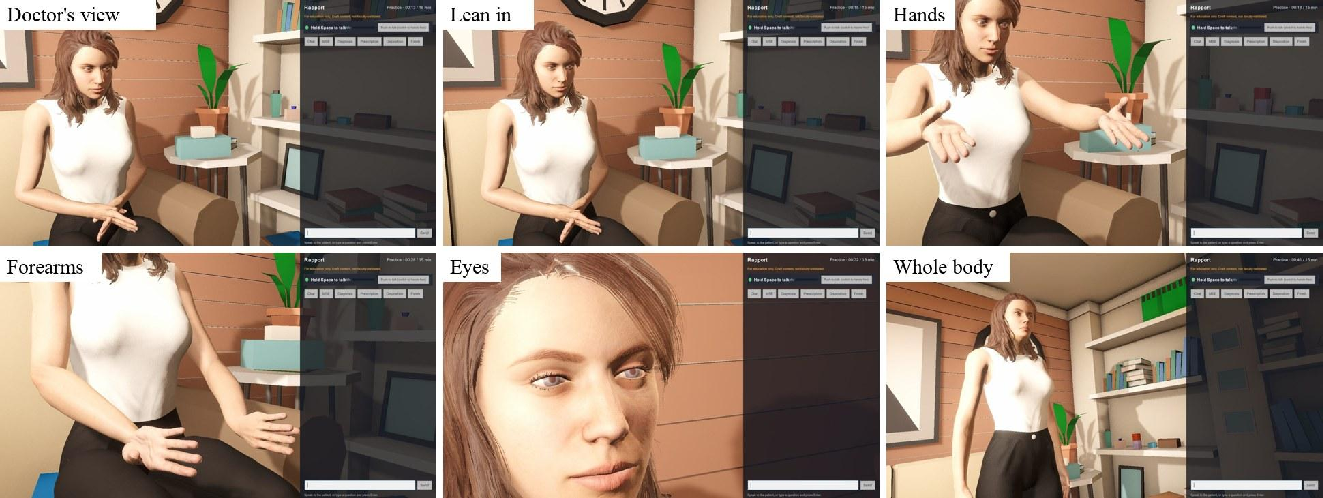
\includegraphics[width=\textwidth]{fig_camera_grid.pdf}
\caption{Camera shots for the doctor's view and the examination close-ups. Stills from the October 2026 build, before the doctor's view was
narrowed to a 30$^\circ$ field of view in v0.3 (Fig.~\ref{p2:fig:stills} shows the current view).}
\label{p2:fig:camgrid}
\end{figure*}

Fig.~\ref{p2:fig:camgrid} shows the shots.

\subsubsection{Lighting}
The room is lit like a bright, warm consulting room. Daylight comes through a window (a 5,000\,K key light from the doctor's side), and a warm ceiling lamp adds fill (3,200\,K, baked). A soft rim light separates the patient from the wall. New in this version, a small face light touches only the patient. Indirect light is baked once (two bounces), so only three lights are computed live and only the key light casts live shadows. One
mistake is worth passing on: setting a light's colour from a colour-temperature conversion that returns linear values made 3,200\,K look like
about 2,000\,K, far too orange; the engine's own colour-temperature mode is correct.

\subsubsection{How the patient looks}
Before the rendering pass, the doctor's camera showed a wide shot with the face only about 67 pixels wide. The faces were darker than the room, and every patient sat turned away: their seat faced about 156 degrees from the doctor. Now the seat faces the doctor at 110 degrees, and the camera frames the patient at conversation distance (face about 142 pixels wide). A soft light that shines only on the patient brightens the face without brightening the room. Face brightness moved into the target range for all four bodies (Fig.~\ref{p2:fig:lum}, Fig.~\ref{p2:fig:stills},
Fig.~\ref{p2:fig:bodies}) with no washed-out pixels. The closer view also revealed that two imported bodies were drawn without hair and eyes from some
angles, because their size boxes were wrong; they are now computed from the skeleton. Rendering one frame at 1920$\times$1080 took 6.4--8.1\,ms in
the editor. The 60-frames-per-second check in the finished app, during a live conversation, has not been run yet.

\begin{figure}[t]
\centering
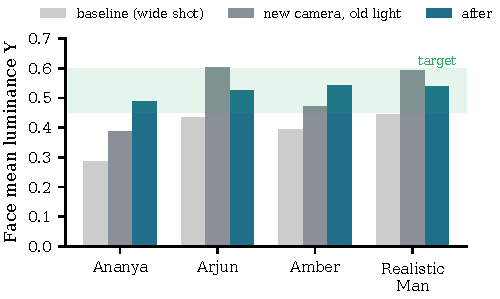
\includegraphics[width=\columnwidth]{fig_luminance.pdf}
\caption{Face brightness of the four bodies; green band: target.}
\label{p2:fig:lum}
\end{figure}

\begin{figure*}[t]
\centering
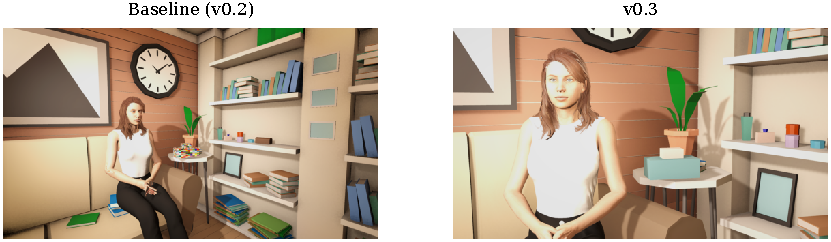
\includegraphics[width=\textwidth]{fig_stills.pdf}
\caption{The doctor's view before and after the rendering pass (same body).}
\label{p2:fig:stills}
\end{figure*}

\begin{figure}[t]
\centering
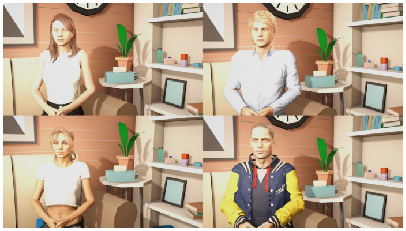
\includegraphics[width=\columnwidth]{fig_bodies.pdf}
\caption{All four bodies from the doctor's seat after the rendering pass.}
\label{p2:fig:bodies}
\end{figure}

\subsubsection{Failures we found, and what they teach}
\begin{itemize}
\item \textbf{Two programs sharing one model slot mixed up replies.} During one test, a replay script and a timing benchmark used the same model server and the same reserved slot at the same time. Replies went to the wrong program. A live session has only one client, so students were
not affected, but test runs must never share the patient's model server.
\item \textbf{Typed turns forgot everything}, as described above.
\item \textbf{The timing benchmark crashed} when the service decided the doctor had finished before the recorded sentence ended; it now records
this as an ``early turn end'' and carries on.
\item \textbf{The voice changed speaker mid-reply}, because the voice description changed between sentences.
\end{itemize}

\subsubsection{Software quality}
The patient service has 244 automated tests, including one for each defect found by the independent safety review; the Unity client has 55
editor tests. Four architecture decisions are written down with their reasons and the options rejected. They cover the Digital Twin's split between code and model, turn detection (Smart Turn adopted, a larger voice-agent framework not), the product name, and the learning loop. Every brain version can be rolled back with one command, and the old brain's tests still pass when it is
live.


\subsection{How the system developed}

\begin{table}[t]
\caption{How Rapport developed (2026)}
\label{p4:tab:history}
\centering
\scriptsize
\begin{tabularx}{\columnwidth}{@{}lY@{}}
\toprule
Version (date) & What changed, with key numbers\\
\midrule
Twin 0.1 (20 Oct) & Live Digital Twin; median wait 3.0\,s $\to$ 1.6\,s\\
v0.2 (21 Oct) & Exam rules (385 sentences, 100\%); expressive voice; learning loop (one learned version rejected for a safety flag)\\
v0.2.1 (22 Oct) & New demo interview; three recall bugs found and fixed\\
Personalities (22--31 Oct) & Seeded patients, six styles, ward events, alcohol case, scoring overhaul, life stories\\
v0.3 (13--14 Nov) & Code decides before the model; meaning-based recall; memory of the conversation; checks before speech; body language;
conversation-distance camera\\
\bottomrule
\end{tabularx}
\end{table}
Table~\ref{p4:tab:history} shows how the system developed, from the first live Digital Twin to the version evaluated here.


\section{Discussion}\label{sec:disc}

\subsection{What the design achieved}
Moving the patient's decisions into code made its behaviour something an examiner can watch, a reviewer can test and a researcher can argue
about. Safety rules became automatic gates, and an independent reviewer could try to break them, and did; all ten defects it found were fixed
and turned into tests before the results were measured. The ablation shows where the safety result comes from: without the decision rubric the
patient failed four jailbreak attempts and fell back to the old, narrow pattern of behaviour (Table~\ref{p1:tab:ablation}). The patient's behaviour
now changes with the kind of doctor it faces, while each single conversation stays as focused as before. Because the patient is data, a new
station is a new file rather than new code, and because the body reads the same decision as the voice, posture, gaze and face agree with what
the patient says. All of this runs on one laptop, so no student's voice leaves the device.

\subsection{What fell short}
\textbf{Accuracy did not rise.} The composite measures accuracy against the case, not realism, and the previous Twin was already accurate.
Whether the added fit to the situation feels more real is a question for clinicians; a blind A/B page with ten pairs of replies is ready but not
yet rated.

\textbf{Recall of reworded risk questions} reached 72.7\% on the held-out half, against a 95\% target. The same method scored 90.7\% on the tuning
half, so a tuning half that is also used to write examples gives a badly over-optimistic number. Tuning only to find more risk questions made the
patient talk about suicide when asked about sleep, which is why recall must be tuned with a limit on wrong matches.

\textbf{An angry patient calmed down too soon.} The upset style was in character on half of the turns after turn 10, because the softening rules
let a consistently kind doctor lower resistance. A minimum hold time for upset patients is the obvious fix.

\textbf{Speed.} A median of 1.8\,s is close to the thoughtful pause of a low-mood patient, but misses a 1.2\,s target for brisker cases. Holding
a whole reply back on a risk turn, so that a denial can be replaced, and the longer prompt both cost time; part of the increase is not yet
traced.

\textbf{Rules that read the doctor.} Word patterns miss some judgemental sentences, such as ``Are you sure you're not just making this up?'', and
the rule against a flat ``No'' on locked topics also fired for an accusation about a non-risk topic, where a plain ``No'' would be natural
(Table~\ref{p1:tab:example}).

\subsection{Lessons for builders}
\begin{enumerate}
\item Keep everything a clinician would audit outside the language model, and give the model a closed list to choose from.
\item Check every sentence before it is spoken, and hold back a whole reply when a single sentence could break a safety rule.
\item Write recall test questions \emph{blind}, from what the memory means, never from the matching rules; keep a test half that is never
touched, and report it rather than the tuning half.
\item Always report wrong risk matches next to risk recall, and use a stricter ``clearly asked'' level for anything with consequences, such as
forcing a disclosure.
\item Let a learning loop change only how the patient speaks, never the case, and gate every learned version on the held-out safety checks; in
our first round the loop was most useful as a test that found bugs.
\item Test with a person early: one playtest found four problems that every scripted test had missed.
\end{enumerate}

\subsection{Limitations and threats to validity}
\begin{itemize}
\item Only four draft stations; psychosis, mania and anxiety are not covered. All clinical content, trust levels and debrief cut-offs are drafts
that psychiatrists must still review.
\item The held-out conversations and the examination tests were written by the developer, and the recall benchmark by a single AI writer, whose
phrasing may be more regular than a nervous student's. The tuning and test halves come from the same writer, so the test half measures new
wording, not a new writer.
\item The judge is a language model and its flags were checked by the developer, not by faculty. LLM judges are known to be biased
\cite{zheng2023judging}.
\item \emph{Construct:} the composite measures accuracy, not realism, and the variety measures count labels, not how a reply feels.
\emph{Statistical:} 36 and 6 runs per version detect large differences only; about 75 risk pairs per benchmark half make each recall figure
uncertain by several points.
\item \emph{External:} two cases in the held-out runs, scripted doctors, one variety of English, one high-end laptop. The student's own body
language is not assessed.
\item The Twin is inspired by brain science but is not a model of the brain.
\end{itemize}

\subsection{Ethics}
No human participants or real patient data were involved. A student's words never become patient facts, and student sessions are used for
learning only with consent. Suicide-related content comes with a content note and a debrief with teaching points. Patient voices are designed
from written descriptions, not copied from real people. Release builds refuse unreviewed clinical content, and demonstrations that use
pre-scripted replies must say so.

\subsection{Next steps}
Table~\ref{tab:next} lists the next steps, in order.

\begin{table}[t]
\caption{Next steps}
\label{tab:next}
\centering
\scriptsize
\begin{tabularx}{\columnwidth}{@{}YY@{}}
\toprule
Step & Why\\
\midrule
Faculty review of all four cases and the flagged replies & Clinical truth and judge accuracy\\
Faculty blind A/B ratings & Answer RQ3: does it feel real?\\
Ethics approval and a student pilot (n $\approx$ 20--30) & Answer RQ5: does it help?\\
Hand-checked labels and a fine-tuned recall model & Reach 95\% recall on risk questions\\
Learned move rules and a hold time for upset patients & Fewer missed judgements; anger that lasts\\
A psychosis or anxiety case & Broader coverage\\
Lip sync and skin, eye and hair shading & A more lifelike face up close\\
\bottomrule
\end{tabularx}
\end{table}

\section{Conclusion}
A spoken, embodied psychiatric standardised patient can run privately on one laptop if the patient is data, code makes the decisions, a local
language model supplies the words, and the body reads the same decision as the voice. With this split, safety becomes a set of checks that anyone
can run and try to break, and the remaining gaps, such as recall of risk questions asked in new words and keeping an angry patient angry, become
measurable targets instead of impressions. Whether the patient is real enough, and useful enough, to teach with is the next question, and it
needs psychiatrists and students to answer it.

\appendices
\section{What a seed changes}
A seed picks one option for each everyday ``slot'' in the case and one conversation style allowed by the case. For the depression case the slots
include a hobby (for example Carnatic singing or badminton), a younger brother's name and a home town; every option is written by hand, so
nothing clinical can change. The answer key, the memories' trust levels, the rating-scale scores and the risk items are the same for every seed.
Assessment mode uses the authored style for every student so that marks are comparable; practice mode allows any style.

\section{Instructions given to the benchmark writer}
The writer received, for each case: the patient's name, age and situation; for each memory its id, its kind (complaint, symptom, history, risk,
social, belief) and a one-line description of what the patient knows; and these rules: write lines a real doctor might say to this patient;
at least 4 per memory and 12 per risk memory; mix textbook, gentle and indirect, clumsy and leading, colloquial Indian English, and euphemistic
phrasings; most lines should avoid the memory's obvious key words; each line must make sense on its own; label each line with every memory it
asks about, and nothing more; include greetings, small talk and empathy-only lines that ask about nothing; mark hard lines. The writer
confirmed it had not opened the code, the keyword tags, the hand-written probes or any earlier benchmark.

\section{Hand-set heads: example questions}
Each head is the normalised average of its example questions' vectors. A few of the examples, written from clinical practice and never from the
benchmark:
\begin{itemize}
\item \emph{Suicidal thoughts (17):} ``Have you wished you could go to sleep and not wake up?'', ``Do you sometimes feel everyone would be better
off without you?'', ``When it gets very heavy, do thoughts of death come to you?''
\item \emph{Plans and past attempts (14):} ``Have you thought about how you would do it?'', ``Have you done anything to prepare, like writing a
note?'', ``Can you keep yourself safe if you go home today?''
\item \emph{Means (12):} ``Have you been saving up medicines?'', ``Can you get onto a roof or somewhere high easily?'', ``Is your home safe for
you right now?''
\item \emph{Harm to others:} ``Has anyone at home been afraid of you?'', ``Have arguments ever got physical?''
\end{itemize}

\section{System requirements and reproducing the results}
\textbf{Hardware and models.} Apple M5 Pro, 24\,GB memory. Patient: Gemma 4 E4B, 4-bit (Q4\_K\_M), llama.cpp server with Metal, flash
attention, all layers on the graphics chip, two parallel slots. Judge: Qwen3.5-9B on a second server. Recall: bge-small-en-v1.5, ONNX, on the
processor. The voice model alone peaked at 8.1\,GB in the bake-off, so a machine with less memory may not fit the expressive voice alongside the
language model.

\textbf{Held-out runs.} For each version $v\in\{\text{v0},\text{v2}\}$, case and seed, run
\texttt{tools/learning/loop.py heldout $v$ --case $c$ --seeds 11,23,42} with the judge URL; \texttt{papers/analysis/analyses.py} computes the
pooled and per-conversation numbers, intervals and decision counts, and \texttt{papers/figures/make\_figures.py} draws the figures.

\textbf{Recall.} \texttt{tools/recall\_bench.py --split test} prints recall and wrong-match rates for the shipped settings; \texttt{--lexical}
gives the keyword baseline and \texttt{--hand} adds the hand-set heads. \texttt{papers/analysis/analyses.py --recall} and
\texttt{recall\_extra.py} compute the by-case, difficulty, probe-source, rank, interval and timing results.

\textbf{Speed.} \texttt{tools/latency/ws\_bench.py} plays synthesised Indian-English doctor lines into the real session connection as 32\,ms
frames and never uses the microphone; results come from the service's own timing log.

The held-out scripts, case files, brain versions, benchmark and its split, and every judged reply are kept with the code, so each number in this
article can be traced to the data behind it.

\section*{Acknowledgment}
\textbf{Use of AI tools.} The text of this article, its figures, tables and analysis scripts, and the \LaTeX{} source were drafted with an AI
assistant (Claude, Anthropic, used through Claude Code), working from the project's code, experiment logs and result files under the author's
direction. The same assistant helped write the software described here, ran the analyses, and checked the citations against their sources.
Within the study itself, AI models were also used as research tools, as described in Section~\ref{sec:eval}: a separate language model
(Qwen3.5-9B) marked the held-out replies, an AI agent wrote the blind recall benchmark, and another AI agent carried out the independent safety
review. The author takes full responsibility for the content of this article.

\bibliographystyle{IEEEtran}
\bibliography{../shared/refs}

\end{document}
